\subsection{Visual Features in Variational Autoencoders}\label{subsec:results_visual_features_in_variational_autoencoders}
The following sections describe the results of the experiments on visual features in variational autoencoders.

\begin{itemize}
    \item Results non-AlexNet-like-VAE on CelebA: especially layer 1 kernels
    \item Results AlexNet-like-VAE on ImageNet: especially layer 1 kernels
    \item Results AlexNet-like image classification CNN on ImageNet: especially layer 1 kernels
    \item Results AlexNet-like-VAE with frozen decoder from classification network
\end{itemize}

\subsubsection{AlexNet Image Classification}
To make sure that the network structure of the \ac{VAE} is apt to generate Gabor wavelets, image classification was performed on ImageNet (see Figure~\ref{fig:alexnet} and Section~\ref{subsec:visual-features-variational-autoencoders} for the used network, see Section~\ref{ssec:imagenet} for ImageNet).
As the accuracy was not of primary concern, the training was stopped during the tenth epoch (\textbf{If time: train all 100 epochs}), the top-1 training accuracy at this time was at 0.85.

\begin{figure}
    \centering
    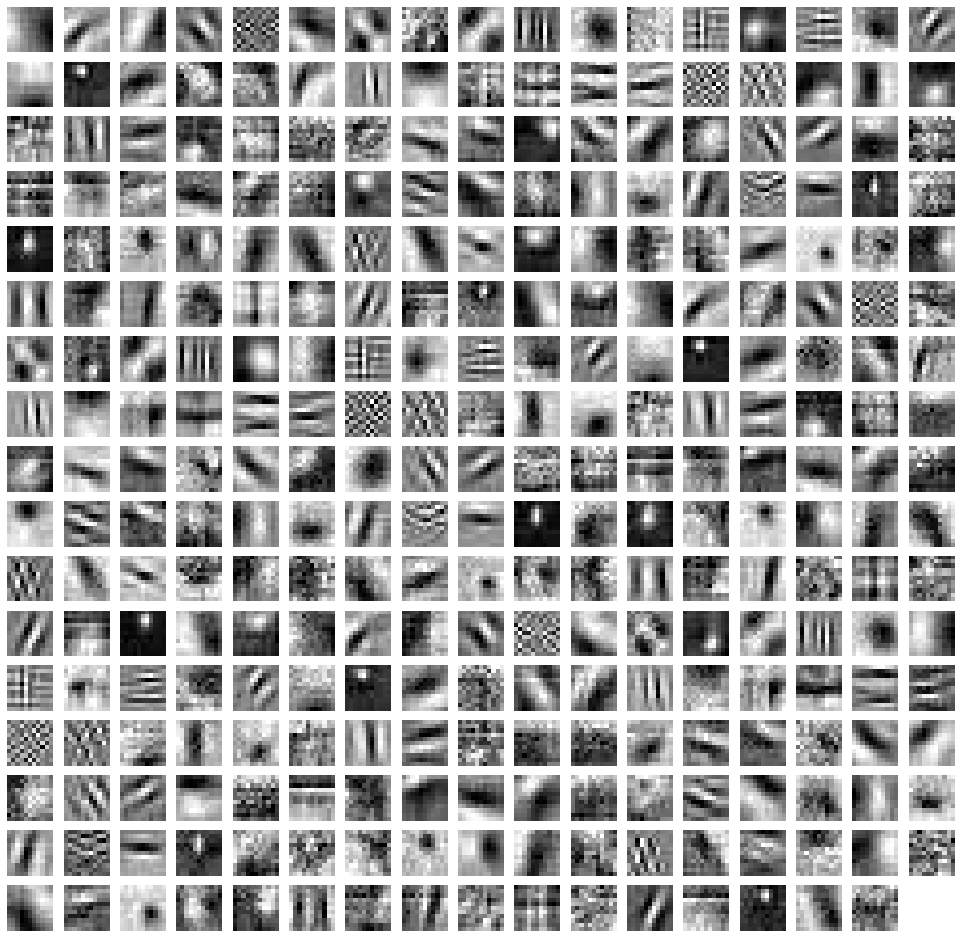
\includegraphics[width=0.9\textwidth]{images/alexnet_classification_l1_kernels.png}
    \caption[Image classification - Layer 1 Kernels]{Convolutional Kernels in the first layer of the image classification network. The filters are shown in their original size (11x11).}
    \label{fig:classification_layer1_kernels}
\end{figure}

Figure~\ref{fig:classification_layer1_kernels} shows all 256 convolutional kernels of the image classification network.
It is easy to see that in many kernels, Gabor wavelet-like filters emerge.

\subsection{Sparseness in Generative Models}\label{subsec:effective-network-capacity}
One hyperparameter to choose in the different models is the number of feature maps of one layer.
During the implementation it could be observed that some feature maps show little activity compared to others, posing the question by how much the number of feature maps can be reduced without increasing the network loss.

Furthermore, the questions arises whether sparseness in \acp{VAE} is related to sparseness in the primary visual cortex (see Section~\ref{subsubsec:sparse_representations}).
The brain uses sparseness to represent information - maybe \acp{VAE} use a similar mechanism.
This would be evidence for relatedness of \acp{VAE} to the biological example.

To answer this question, the feature map activity of a \ac{VLAE} on \textsc{Mnist} with input size $28\times 28$ and different numbers of feature maps and nodes in fully connected layers was measured.
By gradually decreasing the network capacity, it was tested whether sparseness arises due to an initial over-capacity of the network or if it arises because the network employs sparseness under all conditions.
Because it re-scales the feature map activity, batch normalization was disabled for this experiment.
To compensate for the potentially longer training convergence, the model was trained for 200 instead of 100 epochs.

\begin{figure}
    \centering
    \begin{subfigure}{.95\textwidth}
        \centering
        % include first image
        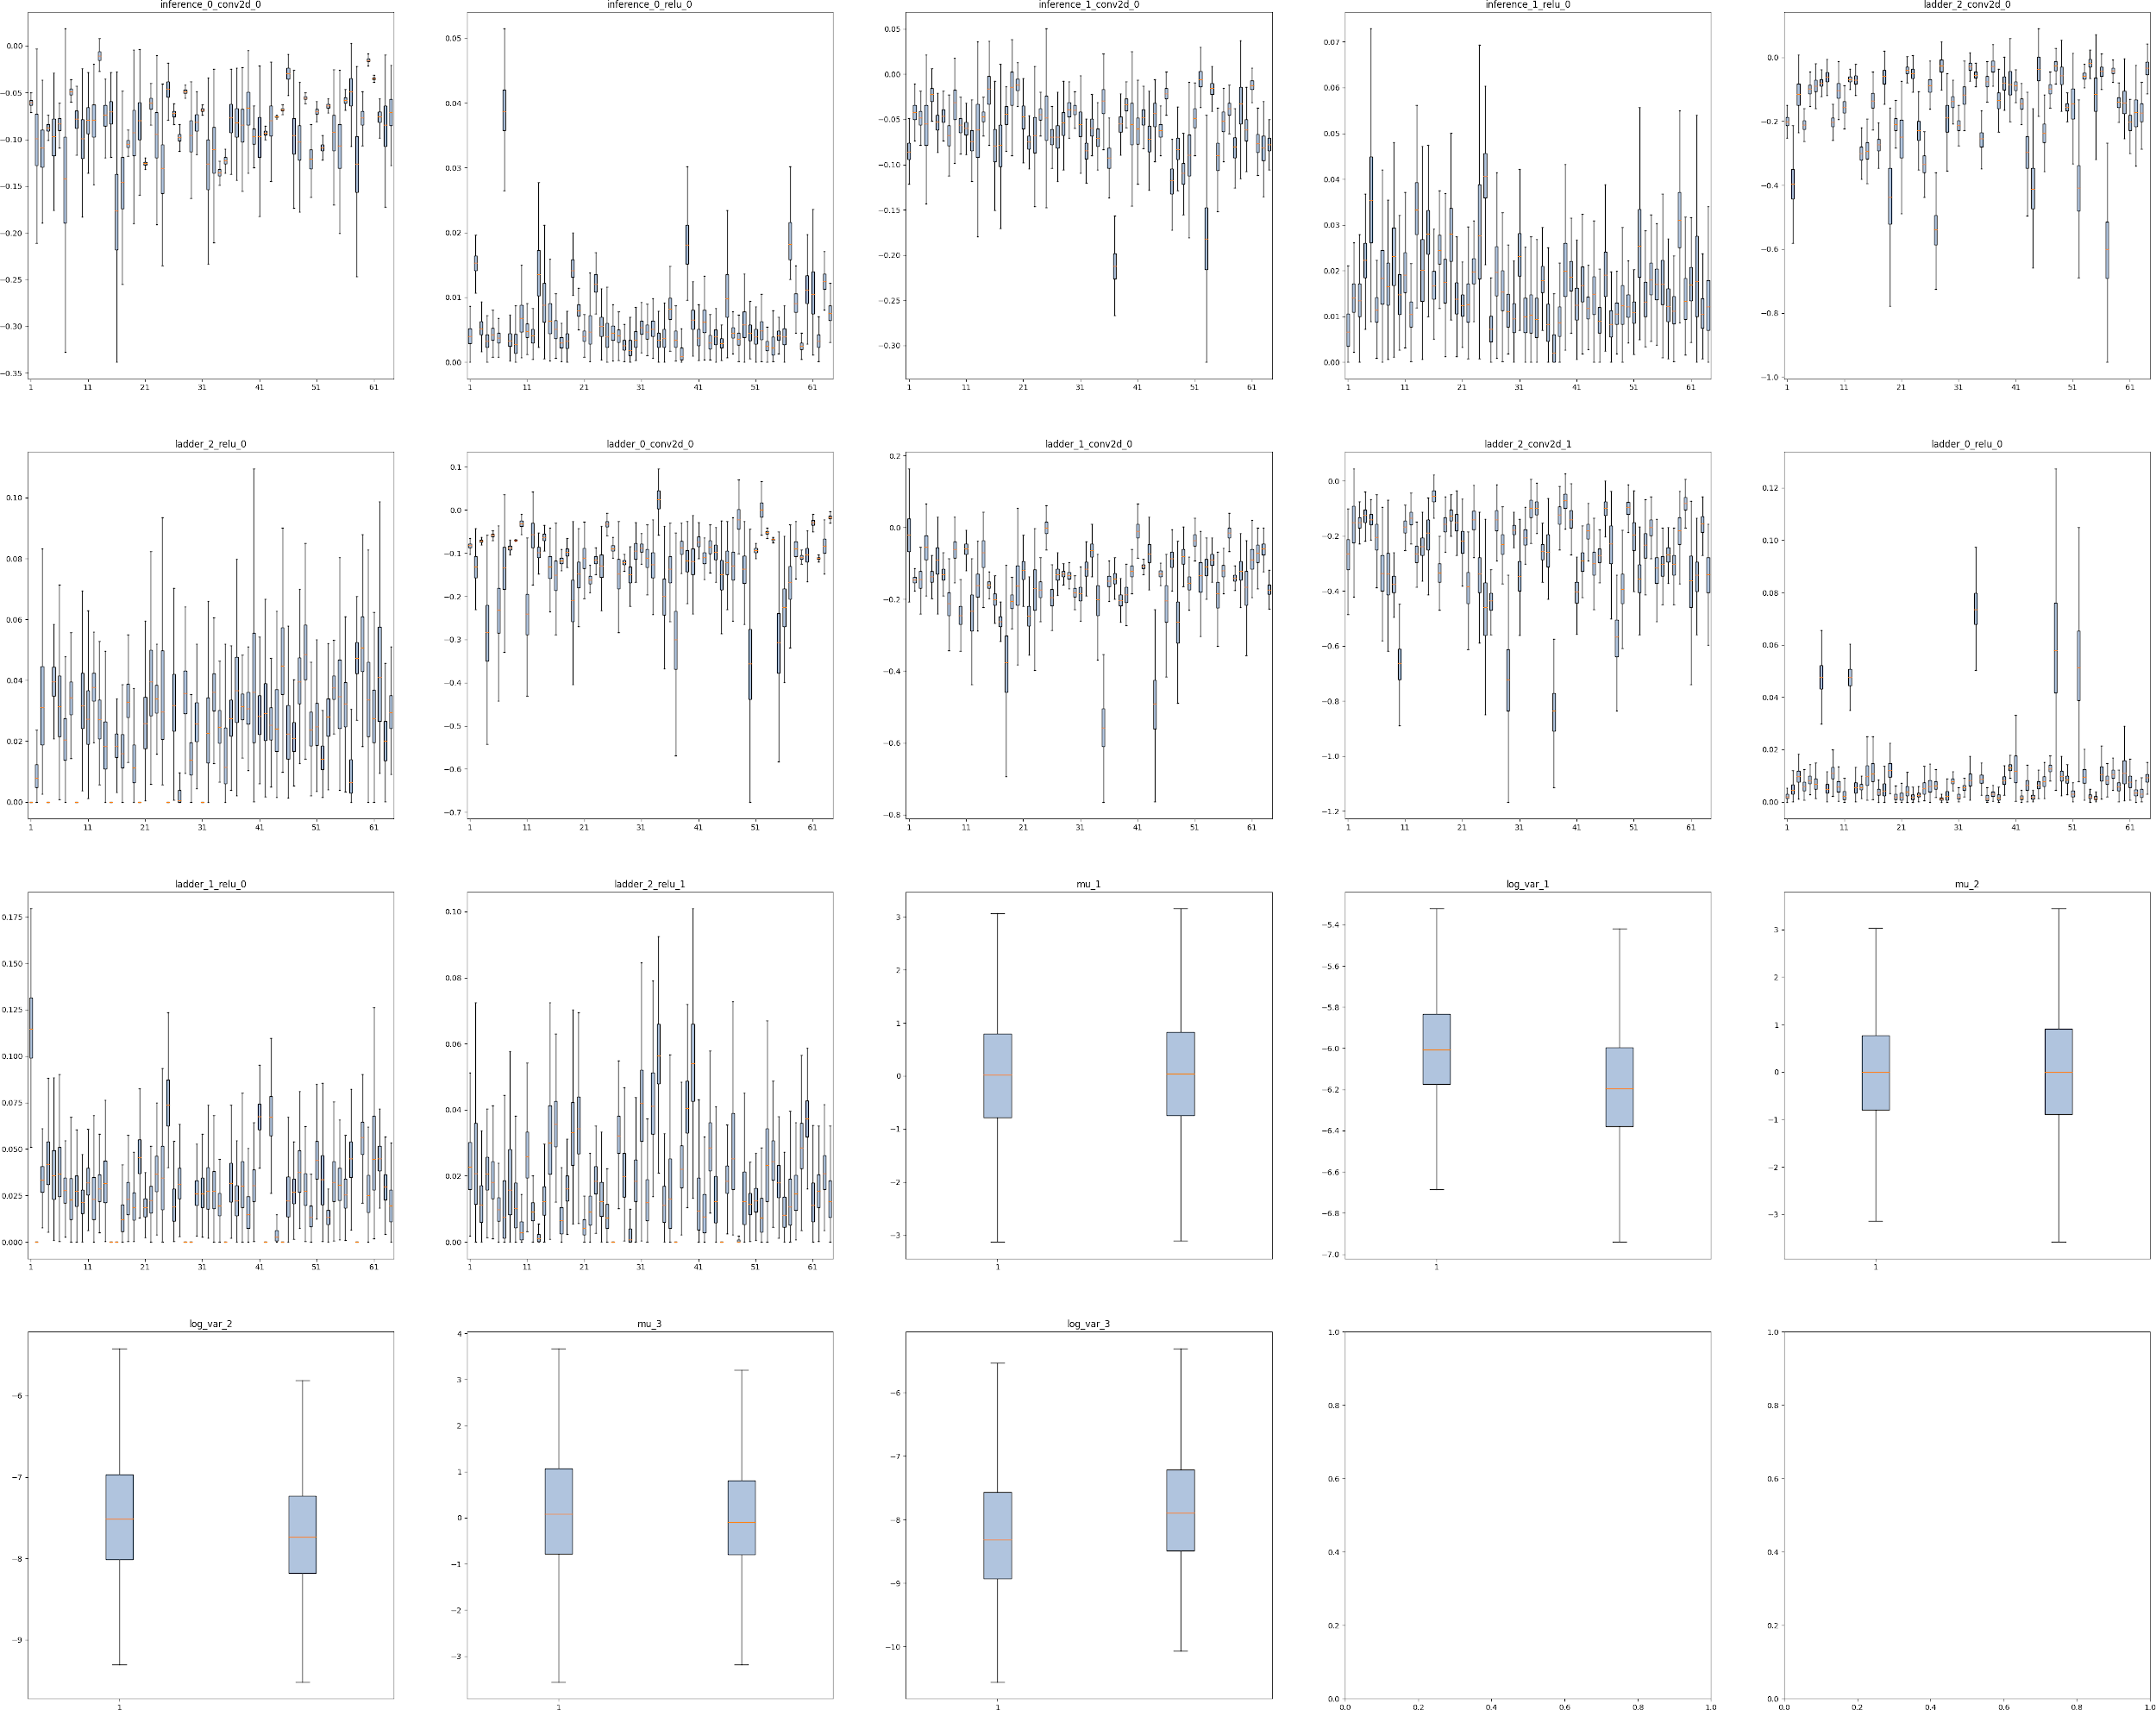
\includegraphics[width=\textwidth]{images/sparseness/encoder_fm1_fms.png}
        \caption{Feature map activities - large model}
    \end{subfigure}
\end{figure}
\begin{figure}
    \ContinuedFloat
    \centering
    \begin{subfigure}{.95\textwidth}
        \centering
        % include second image
        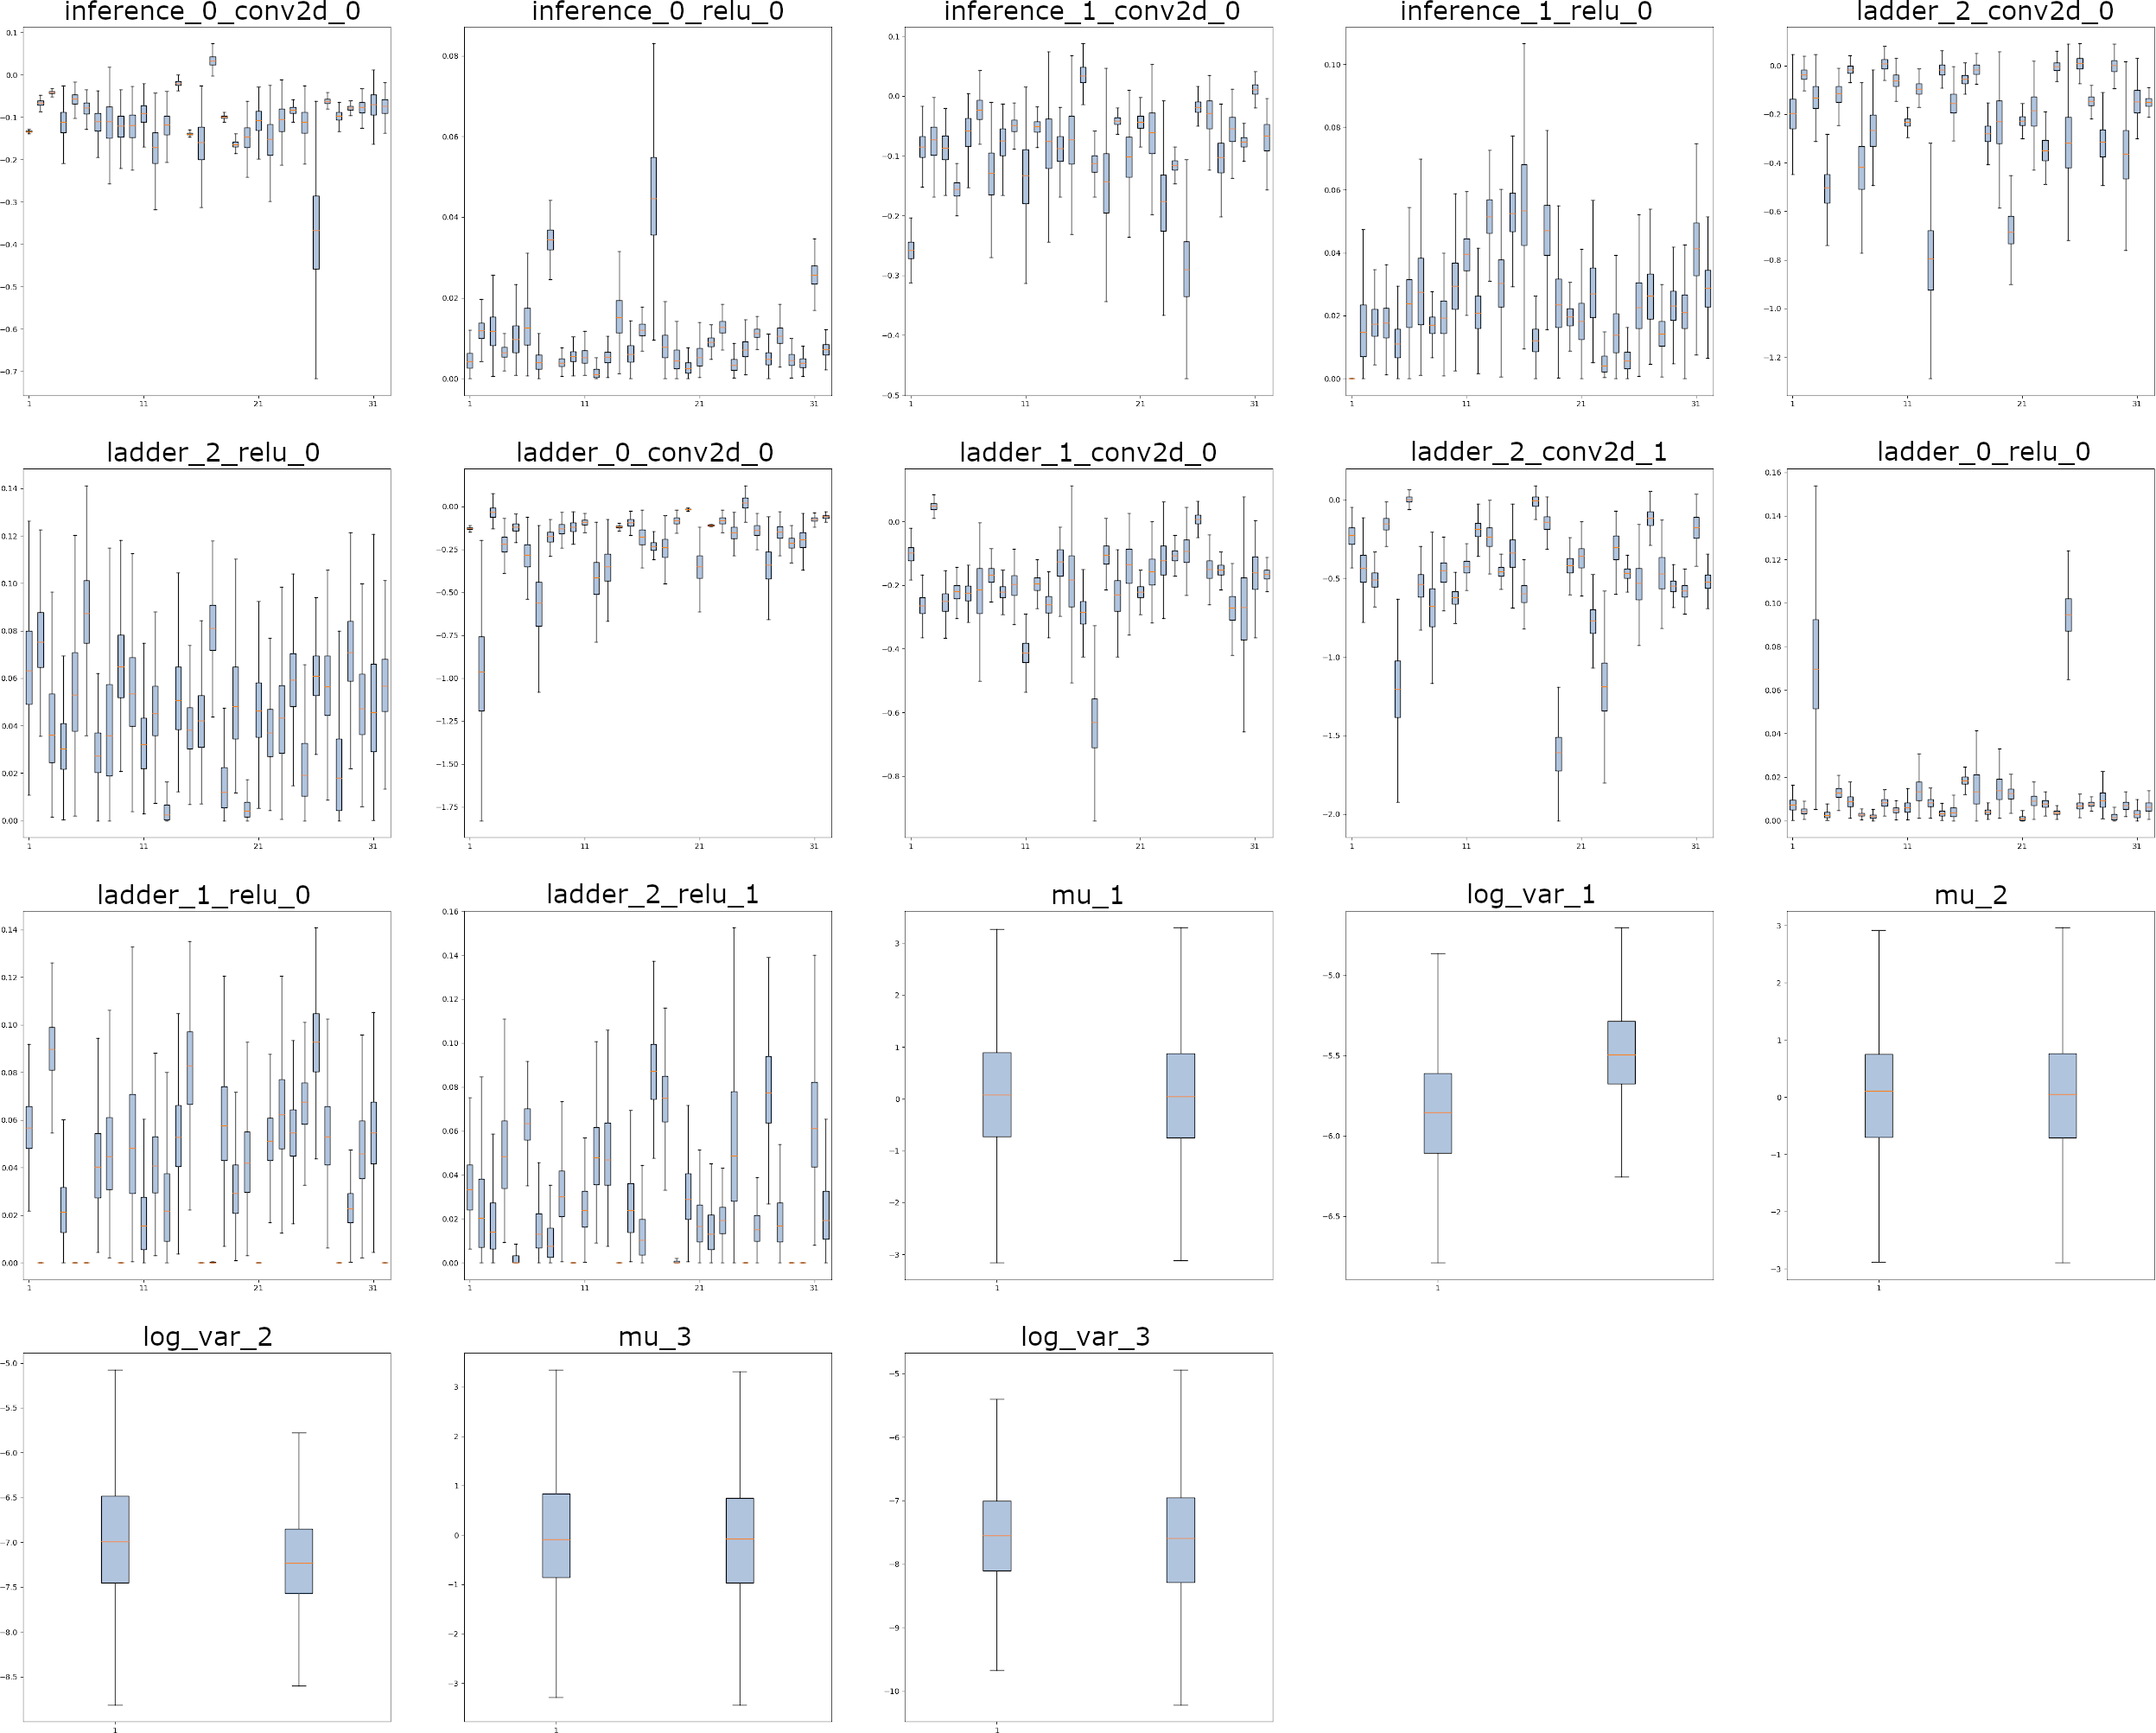
\includegraphics[width=\textwidth]{images/sparseness/encoder_fm2_fms.png}
        \caption{Feature map activities - medium model}
    \end{subfigure}
\end{figure}
\begin{figure}
    \ContinuedFloat
    \centering
    \begin{subfigure}{.95\textwidth}
        \centering
        % include second image
        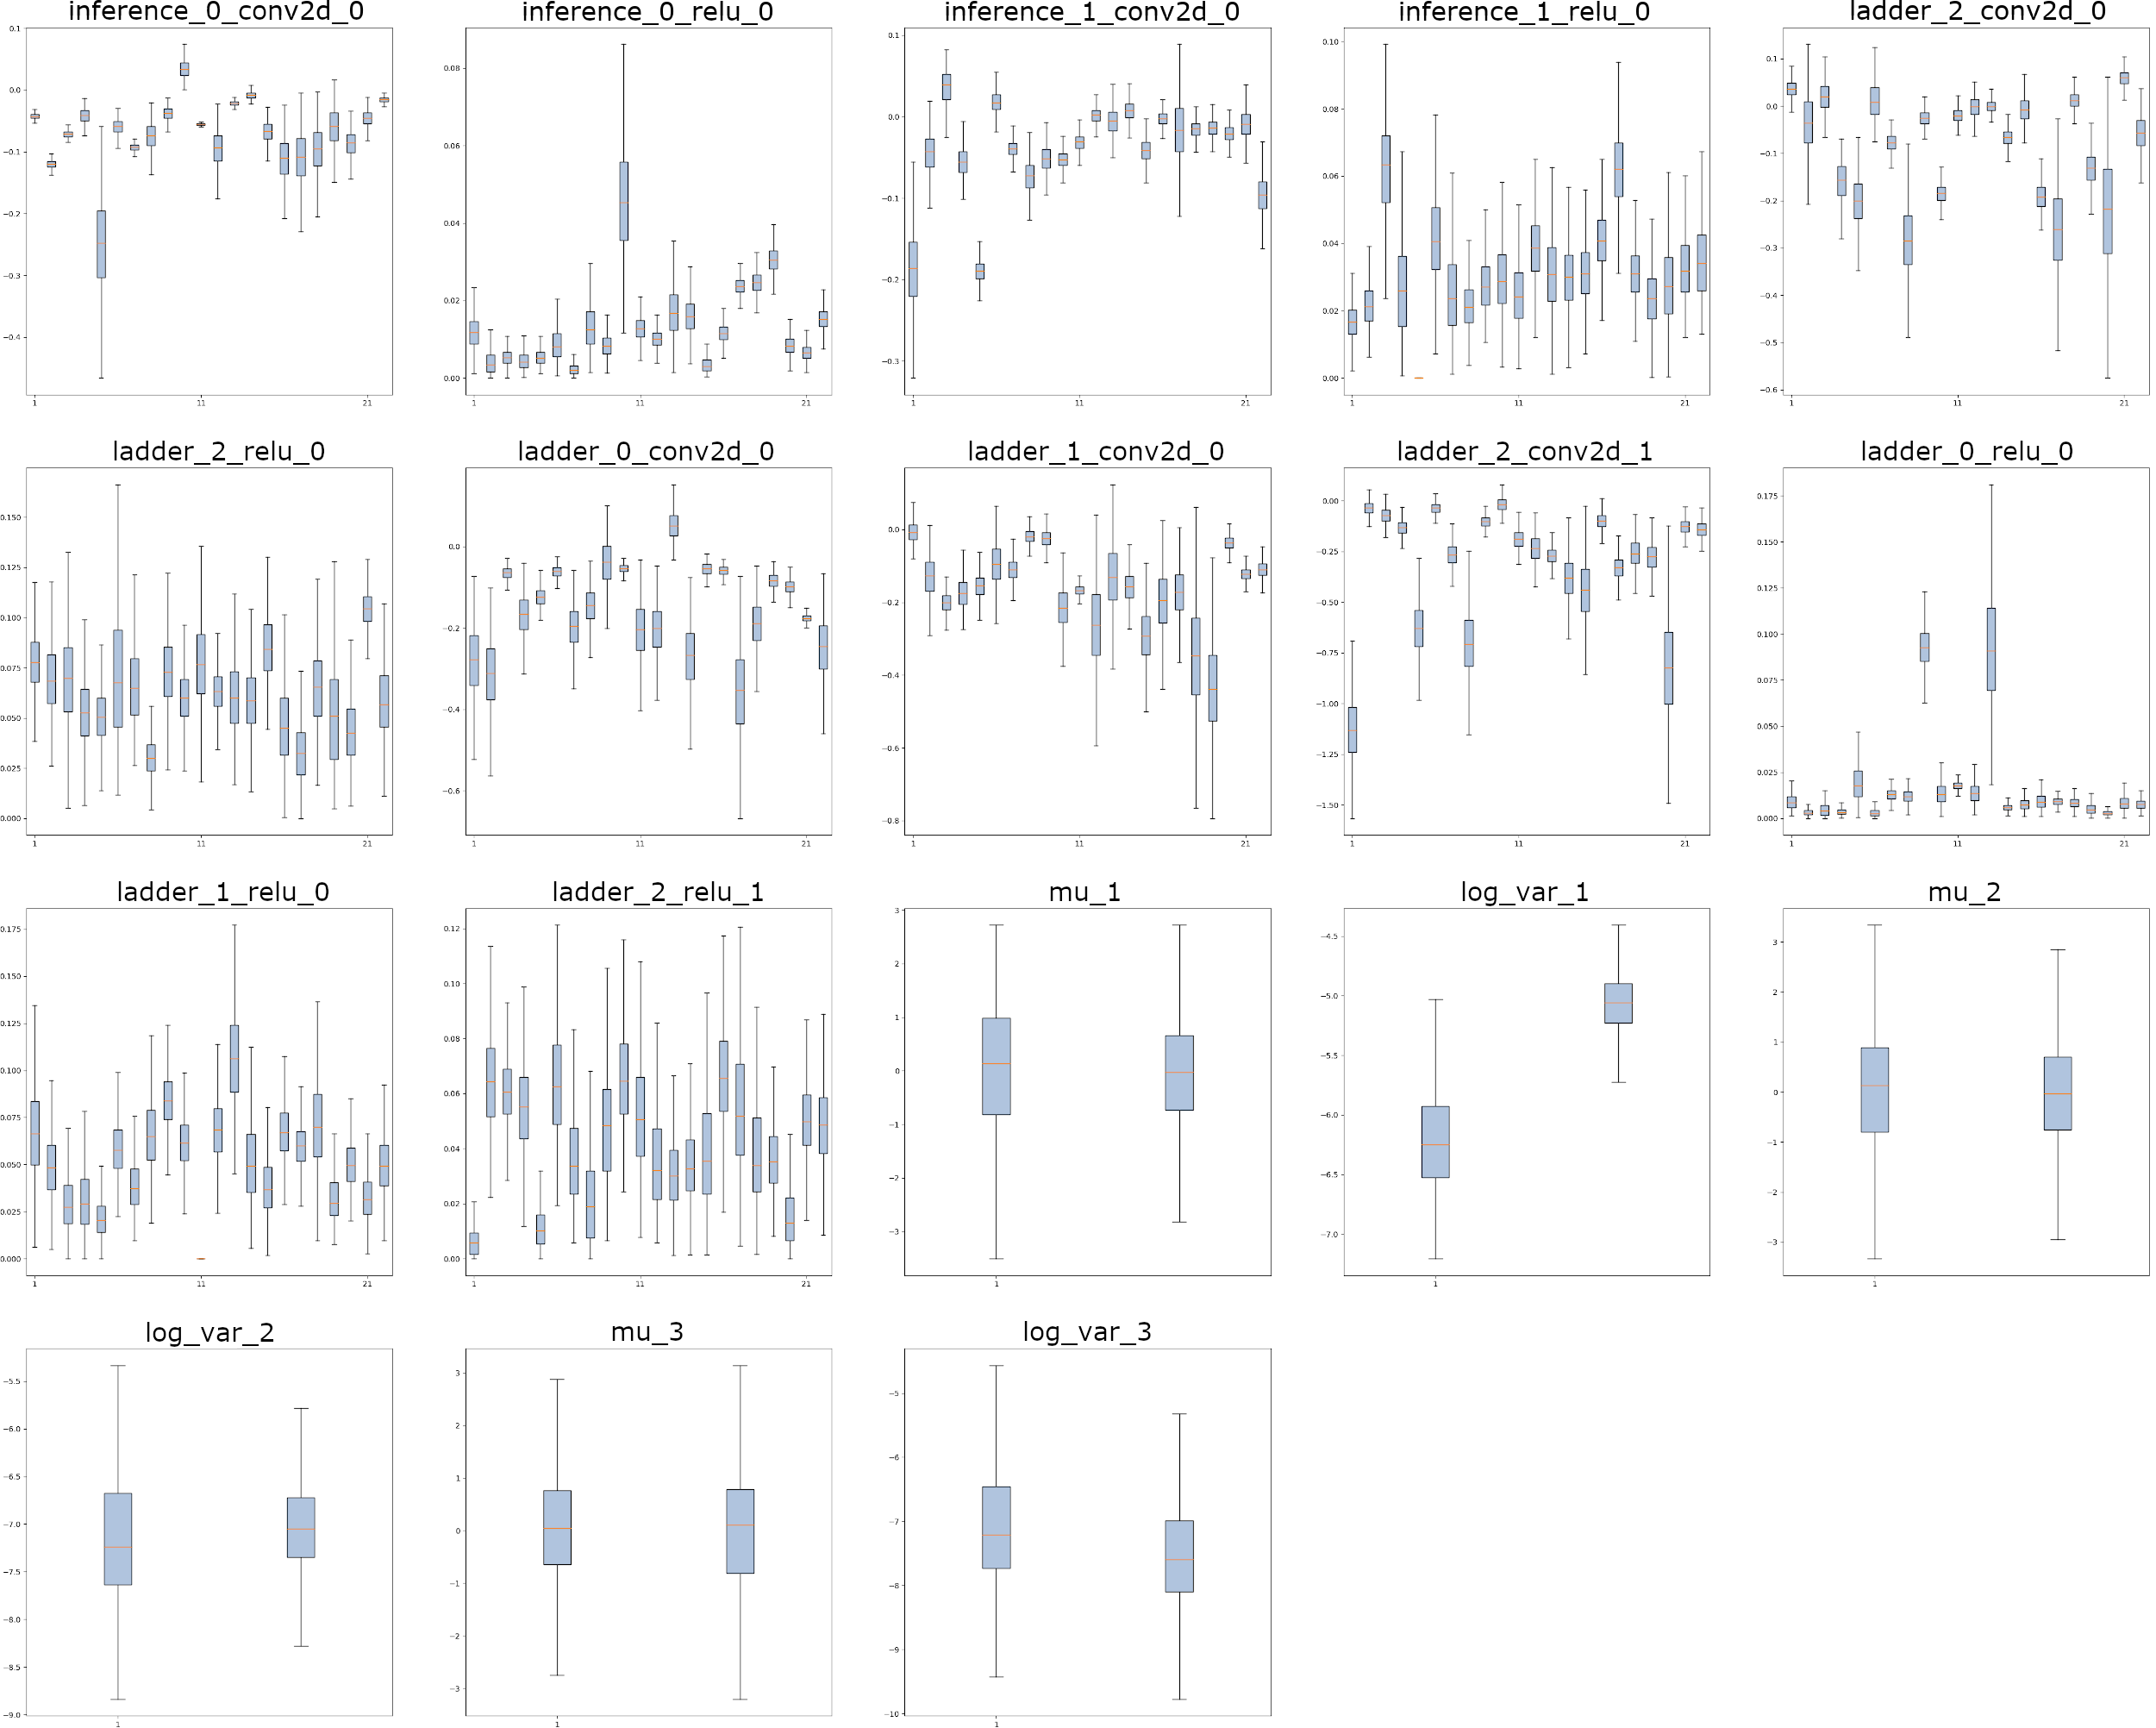
\includegraphics[width=\textwidth]{images/sparseness/encoder_fm3_fms.png}
        \caption{Feature map activities - small model}
    \end{subfigure}
    \caption{Feature map activities for the different models}
    \label{fig:fm_activities_sparseness}
\end{figure}

Listing~\ref{lst:sparsity-vlae-encoder-28-fm1} shows the output of the \ac{VLAE} encoder used for the experiments on sparsity.
Importantly, this is the initial encoder.
Three models were trained in total with a gradually decreased number of feature maps (by the factor of two and three).
All network configurations can be found in Appendix~\ref{sec:listings_sparsity_networks}.
The models were trained with the Adam optimizer with an initial learning rate of 0.0005 for the model with the original number of feature maps\footnote{An initial learning rate of 0.001 for the \say{large} model led to an \textbf{overflow}} and a learning rate of 0.001 for the models of decreased number of feature maps.
All models use a reconstruction loss factor of 10,000 and three two-dimensional latent spaces.
The inner activation function is ReLU in all cases.

\begin{figure}
    \centering
    \begin{subfigure}{.45\textwidth}
        \centering
        % include first image
        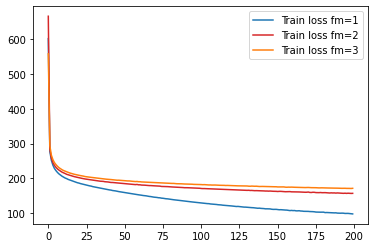
\includegraphics[width=\textwidth]{images/sparseness/sparseness_train_loss.png}
        \caption{Training loss}
    \end{subfigure}
    \hfill
    \begin{subfigure}{.45\textwidth}
        \centering
        % include second image
        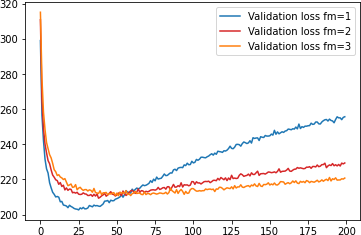
\includegraphics[width=\textwidth]{images/sparseness/sparseness_validation_loss.png}
        \caption{Validation loss}
    \end{subfigure}
    \caption[Sparse Models - Loss Curves]{Loss curves of models with different number of feature maps (see Appendix~\ref{sec:listings_sparsity_networks}). $fm$ is the reduction factor of the feature maps; $fm-1$, therefore, is the original model, $fm=2$ the model with half the number of feature maps, and $fm=3$ the model with one third of the feature maps.}
    \label{fig:learning_curves_sparseness}
\end{figure}

Figure~\ref{fig:learning_curves_sparseness} shows training and validation losses of the different models.
Firstly, increasing the number of feature maps increases convergence speed.
Even though the large model (the model with the original number of feature maps) is trained with a slightly smaller learning rate, it covnerges faster compared to the smaller models.
It, however, does not only converge faster in terms of training loss, it also achieves the lowest validation loss amongst the three models.
The minimum validation loss is achieved faster than the minimum validation loss of the other models.
After achieving the minimum validation loss, however, all models overfit.
The large model overfits stronger than the smaller models, leading to the highest validation loss after 200 epochs.
The validation loss is minimal after 26 epochs for the large, 39 epochs for the medium, and 52 epochs for the smallest model.

Figure~\ref{fig:fm_activities_sparseness} shows the activities of feature maps in the different models.
Each line in a subplot is a boxplot.
Each subfigure is the output of either a convolutional, an activation, or a fully connected layers.
Most prominently, the activations are sparse after convolutions.
The activations usually decrease the level of sparsity.
Nonetheless, sparsity is apparent in almost all figures - in the larger as well as in the smaller models.

\paragraph{Sparsity in \acp{VLAE} vs. Sparse Representations}
The sparseness in \acp{VLAE}, however, does not seem to be related to sparse representations in the brain.

Even though there are only some feature maps showing high activity, they are mostly the same regardless of the input.
This is different from the brain where the overlap of active neurons is small and different neurons are active for different stimuli (see Section~\ref{subsubsec:sparse_representations} and \citet{yoshida2020natural}).

The reason why the \ac{VLAE} uses sparseness, mostly regardless of the model capacity, seems to be more related to the Lottery Ticket Hypothesis~\citep{frankle2018lottery}.
In all cases, there seems to be a subnetwork.
Pruning the original network such that only the subnetwork persists should lead to a comparable performance.
Assume that the small \ac{VLAE}-network approximately is a pruned version of the large \ac{VLAE}-network, having only as many feature maps as are active in the large network.
Then, the small network is not the successful subnetwork in the large network~\citep{frankle2018lottery}.
Instead, the small network itself has a successful subnetwork.

The Lottery Ticket Hypothesis states that it is in general not possible to train the pruned network from scratch without knowing the weight initializations obtained from training the unpruned network.

\subsection{Model Generated Samples}\label{subsec:model-generated-samples}

\subsubsection{Latent Space Traversals}

\subparagraph{\textsc{Mnist}}

A latent space traversal is one way to see if and how a model learns a general representation of the dataset.
Figure~\ref{fig:mnist_latent_space_traversal} shows the latent space traversal of \ac{VAE}, \ac{VAE}-\ac{GAN}, \ac{VLAE}, and \ac{VLAE}-\ac{GAN}.
For the models with only one latent layer (\ac{VAE} and \ac{VAE}-\ac{GAN}), the plot is generated by traversing the latent space in equal steps from $z_i = -3$ to $z_i = 3$ in both dimensions.
For the hierarchical models (\ac{VLAE} and \ac{VLAE}-\ac{GAN}), one $z$-layer was fixed and traversed in the same way.
The values of the other $z$-layers were obtained by sampling from a uniform distribution over $[-3; 3]$.

First, most models properly employ the latent space - the traversal shows almost no non-representative generated images, with a few exceptions for \ac{VLAE} and \ac{VLAE}-\ac{GAN}.
Noteworthy, these non-representative images mainly occur on the borders where the variance is high.
The models were trained such that the latent space is standard normal, the latent space traversal, however, goes from -3 to 3, in areas with low probability density.
Unrepresentative generations in such areas, therefore, is no model failure.

\begin{figure}
    \centering
    \begin{subfigure}{.45\textwidth}
        \centering
        % include first image
        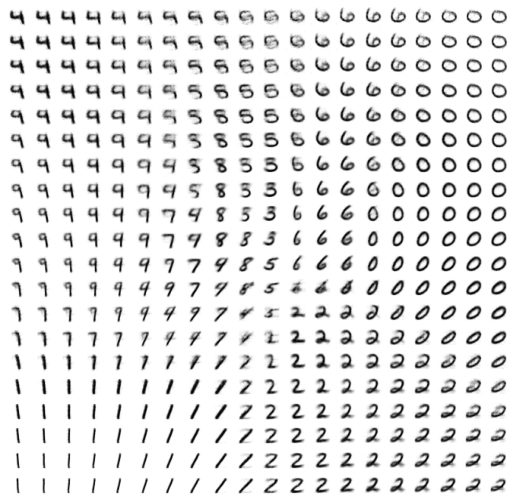
\includegraphics[width=\textwidth]{images/latent_space_traversals/vae_mnist.png}
        \caption{\ac{VAE} latent space traversal from $z_i=-3$ to $z_i=3$ in both $z$ dimensions}
    \end{subfigure}
    \hfill
    \begin{subfigure}{.45\textwidth}
        \centering
        % include second image
        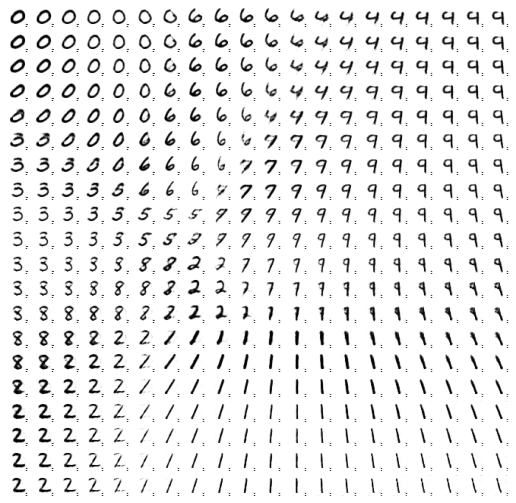
\includegraphics[width=\textwidth]{images/latent_space_traversals/vae_gan_mnist.png}
        \caption{\ac{VAE}-\ac{GAN} latent space traversal from $z_i=-3$ to $z_i=3$ in both $z$ dimensions}
    \end{subfigure}
\end{figure}
\begin{figure}
    \ContinuedFloat
    \centering
    \begin{subfigure}{\textwidth}
        \centering
        % include second image
        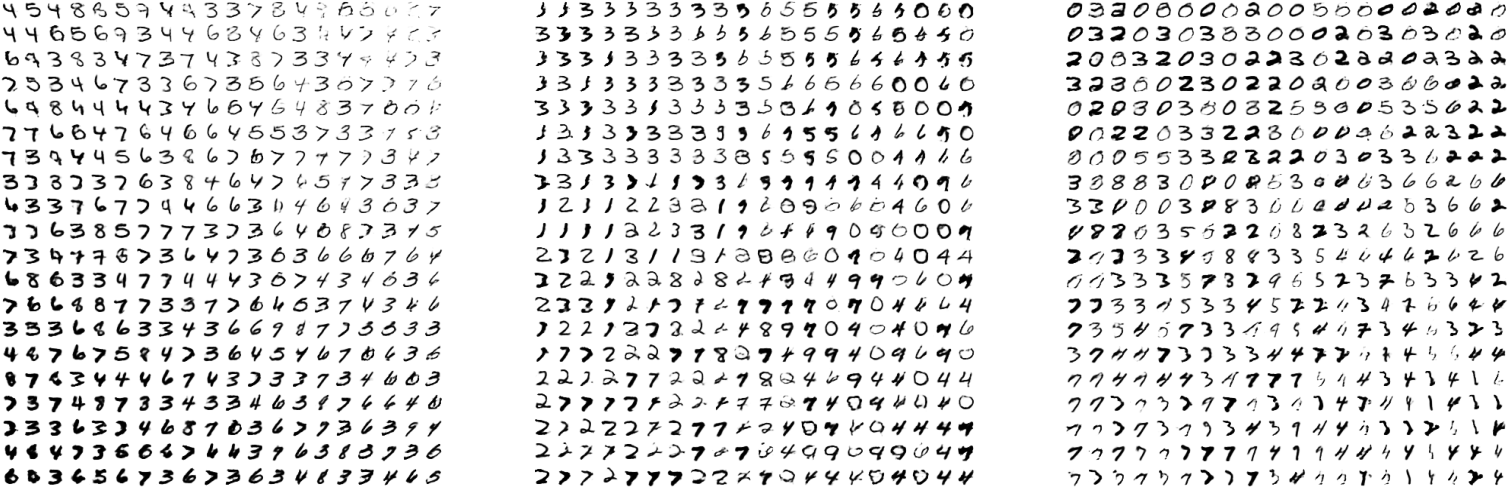
\includegraphics[width=\textwidth]{images/latent_space_traversals/vlae_mnist.png}
        \caption{\ac{VLAE} latent space traversal from $z_i=-3$ to $z_i=-3$ in both dimensions for the respective $z$-dimension. The other $z$ dimensions are sampled uniformly over $[-3; 3]$}
        \label{subfig:vlae_mnist_latent_space_traversal}
    \end{subfigure}
    \begin{subfigure}{\textwidth}
        \centering
        % include second image
        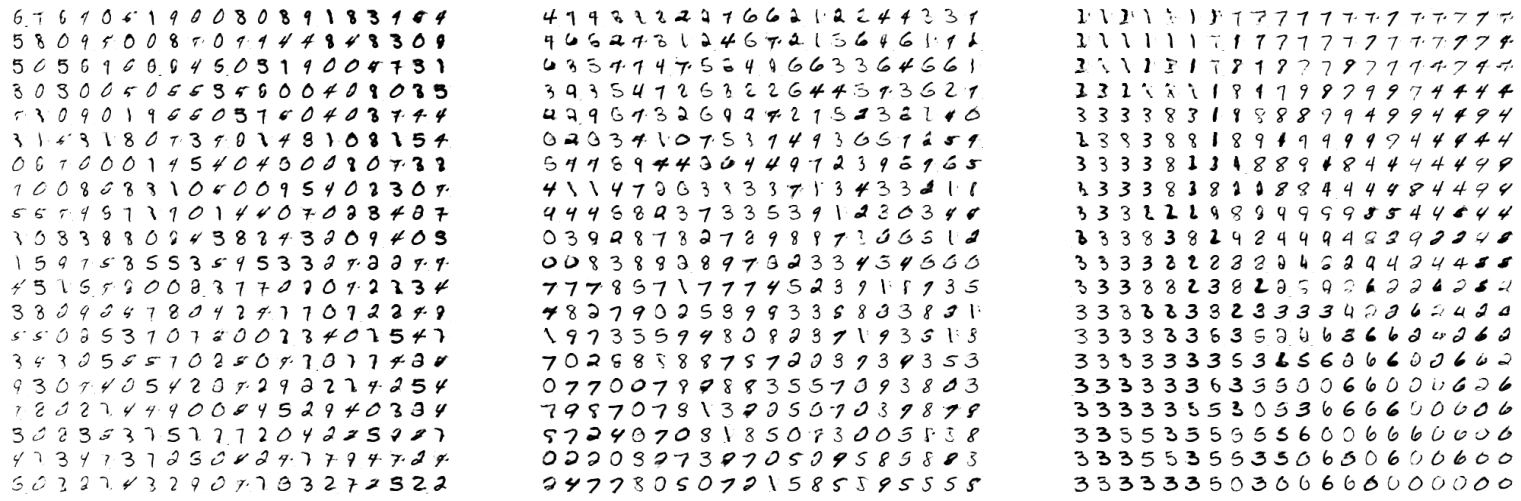
\includegraphics[width=\textwidth]{images/latent_space_traversals/vlae_gan_mnist.png}
        \caption{\ac{VLAE}-\ac{GAN} latent space traversal from $z_i=-3$ to $z_i=3$ in both dimensions for the respective $z$-dimension. The other $z$ dimensions are sampled uniformly over $[-3; 3]$}
        \label{subfig:vlae_gan_mnist_latent_space_traversal}
    \end{subfigure}
    \caption[Models on \textsc{Mnist} - Latent Space Traversal]{Latent space traversal for different models on \textsc{Mnist}. The original images have been inverted for the purpose of this figure.}
    \label{fig:mnist_latent_space_traversal}
\end{figure}

\subparagraph{CelebA}

\begin{figure}
    \centering
    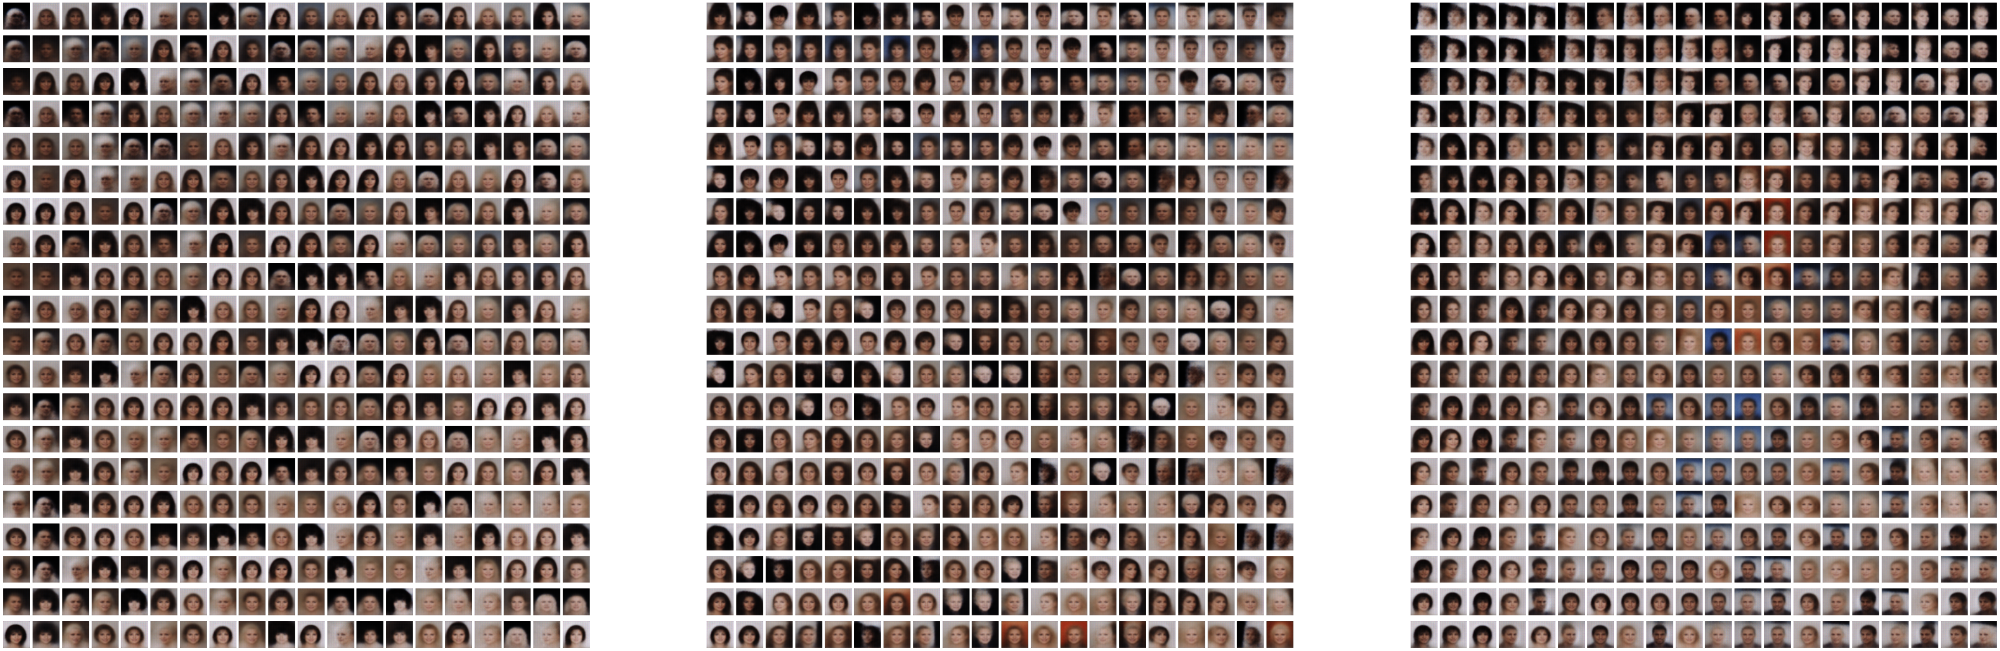
\includegraphics[width=\textwidth]{images/latent_space_traversals/vlae_gan_celeba.png}
    \caption[\ac{VLAE}-\ac{GAN} on CelebA: Latent Space Traversal]{Latent space traversal of \ac{VLAE}-\ac{GAN} with $z_{dim_i}=2$ on CelebA.}
    \label{fig:celeba_latent_space_traversal}
\end{figure}

Figure~\ref{fig:celeba_latent_space_traversal} shows the latent space traversal of a \ac{VLAE}-\ac{GAN} model with input size $128\times 128$ on the CelebA dataset.
The model was generated by evenly interpolating in $[-3; 3]$ in the respective layer and by sampling from a uniform distribution over $[-3; 3]$ for the other layers.
Similar to \textsc{Mnist}, the model learns different factors of variation on different layers.
Layer 1 mainly learns skin color, layer 2 hair color, and layer 3 pose and background color.
Importantly, the model learns only few factors of variation due to the small latent space dimensionality.

\begin{figure}
    \centering
    \begin{subfigure}{\textwidth}
        % include second image
        
\includegraphics[width=\textwidth]{images/latent_space_traversals/vae_celeba_black_to_blond.png}
        \caption{Black to Blond Hair}
        \label{subfig:black_to_blond}
    \end{subfigure}
    \begin{subfigure}{\textwidth}
        % include second image
        
\includegraphics[width=\textwidth]{images/latent_space_traversals/vae_celeba_man_to_woman.png}
        \caption{Female to Male}
        \label{subfig:female_to_male}
    \end{subfigure}
    \caption[Interpolating between black and blond hair, man and woman]{Interpolating between latent factors of variation in a \ac{VAE} latent space, trained on CelebA}
    \label{fig:vae_celeba_black_to_blond_man_to_woman}
\end{figure}

As discussed in Section~\ref{subsubsec:representation_learning}, \textit{feature consistency} is an important of \acp{VAE}.
It was empirically evaluated if the \ac{VAE} models have the same property.
Figure~\ref{fig:vae_celeba_black_to_blond_man_to_woman} shows the transition between black and blond hair, and female and male for a \ac{VAE} trained on imagenet.

To generate the plots, the mean vectors of the different factors of variation (\textit{male}, \textit{black hair}, etc.) were obtained by predicting the posterior for respective images from CelebA.
Then, for Figure~\ref{subfig:black_to_blond} a random latent vector $\bm{v}_1$ with \say{black hair} was chosen from the dataset.
The transition was then generated by choosing different values $\alpha \in [0, 2]$ in the operation $\bm{v}_1 - \bm{v}(\text{black hair}) + \alpha\bm{v}(\text{blond hair})$.
For Figure~\ref{subfig:female_to_male}, a random image was generated by sampling $\bm{v}_2\sim \mathcal{N}(\bm{0}, \bm{I})$.
The transition then was generated by $\bm{v}_2 + \alpha\bm{v}(\text{blond hair})$ with $\alpha \in [0, 4]$.

Even though larger values of $\alpha$ are required to obtain expressive translations, the latent space has the discussed semantic property.
The same holds for \ac{VAE}-\ac{GAN}.

\subparagraph{dsprites}

\textbf{TODO: Plots and Discussion}

\subsubsection{Latent Space Embeddings}\label{subsubsec:latent_space_embeddings}

\paragraph{\textsc{Mnist}}

Figures~\ref{fig:vae_latent_space_mnist} and \ref{fig:vlae_latent_space_mnist} show the latent spaces of \ac{VAE} and \ac{VLAE} trained on the \textsc{Mnist} dataset.
For \ac{VAE}, there is only one latent space while there are three for \ac{VLAE}.
The embeddings are colored by different means, employing information from Morpho-\textsc{Mnist} (see Section~\ref{subsubsec:morphomnist}) and the digit identity information provided by \textsc{Mnist} itself.

As discussed in Section~\ref{subsubsec:representation_learning}, the \acl{VLAE} aims at learning \say{hierarchical disentangled representation}~\citep{zhao2017learning}.
The lower embedding layers of such a model trained on MNIST (see Section~\ref{subsubsec:mnist}) encode features such as stroke width, digit width, and digit tilt whereas the highest layer mainly learns digit identity~\citep{zhao2017learning}.

Incorporating the additional labels provided by Morpho-\textsc{MNIST} (see Section~\ref{subsubsec:morphomnist}) helps to analyze to what extent the lower layers learn which morphological features of \textsc{MNIST}.
The morphological attributes, however, are not equally distributed for all digits.
The mean stroke length and the digith width, for example, have a very low mean value for the digit \say{1} (see Figure~\ref{fig:morpho_mnist_distribution}).
Therefore, it should be possible to almost uniquely identify the identity of the digit \say{1} by just considering the stroke length or the digit width.
Other attributes such as stroke thickness, digit slant, and digit height are more evenly distributed (see Figure~\ref{fig:morpho_mnist_distribution}).

Consider Figure~\ref{subfig:vlae_mnist_latent_space_z_1_slant} showing the embedding layer $\bm{z}_1$ colored by digit slant.
Figure~\ref{fig:morpho_mnist_distribution} shows that the mean of the attribute \textit{Slant} is quite evenly distributed.
The color gradient in Figure~\ref{subfig:vlae_mnist_latent_space_z_1_slant} therefore indicates that the VLAE actually learns the morphological attribute instead of just showing the class identity, encoded by means of another morphological attribute that correlates with class identity.

For Figure~\ref{subfig:vlae_mnist_latent_space_z_1_width}, the situation is different.
The noticeable dark-purple cluster in the top left correlates with dark-purple points in Figure~\ref{subfig:vlae_mnist_latent_space_z_1_identity} that encode image with label \say{1}.
For digit width, however, \say{1} is an outlier (see Figure~\ref{fig:morpho_mnist_distribution}) and a small digit width therefore is a strong indicator for a digit identity of \say{1}.
Nonetheless, overall digit identity does not seem to be encoded strongly by $\bm{z}_1$ (see Figure~\ref{subfig:vlae_mnist_latent_space_z_1_identity}).

\begin{figure}
    \centering
    \begin{subfigure}{.32\textwidth}
        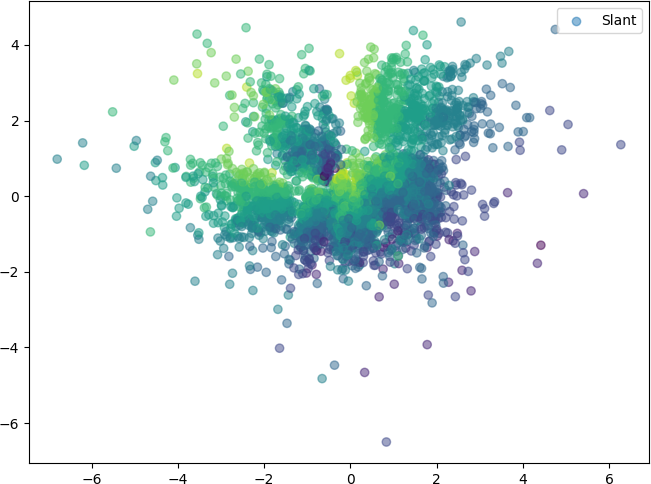
\includegraphics[width=\textwidth]{images/latent_spaces/mnist/vae/embeddings_mu_0.png}
        \caption{Latent space colored by digit slant}
        \label{subfig:vae_mnist_latent_space_slant}
    \end{subfigure}
    \hfill
    \begin{subfigure}{.32\textwidth}
        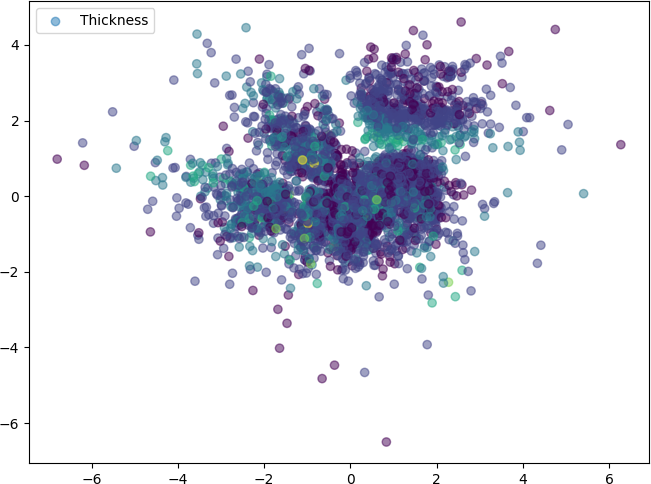
\includegraphics[width=\textwidth]{images/latent_spaces/mnist/vae/embeddings_mu_1.png}
        \caption{Latent space colored by digit thickness}
        \label{subfig:vae_mnist_latent_space_thickness}
    \end{subfigure}
    \hfill
    \begin{subfigure}{.32\textwidth}
        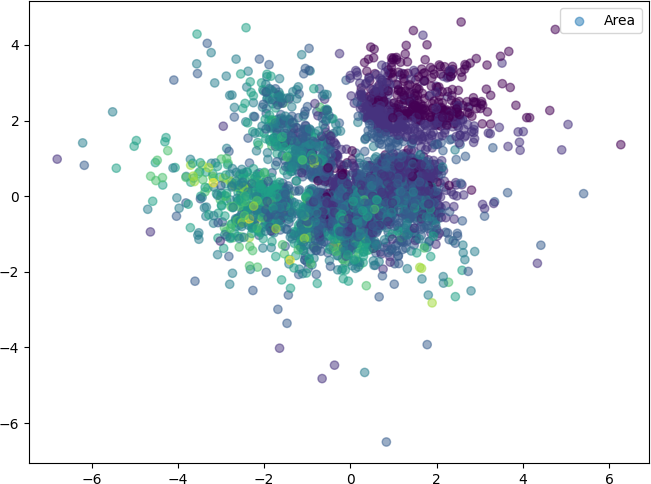
\includegraphics[width=\textwidth]{images/latent_spaces/mnist/vae/embeddings_mu_2.png}
        \caption{Latent space colored by digit area}
        \label{subfig:vae_mnist_latent_space_area}
    \end{subfigure}
    \hfill
    \begin{subfigure}{.24\textwidth}
        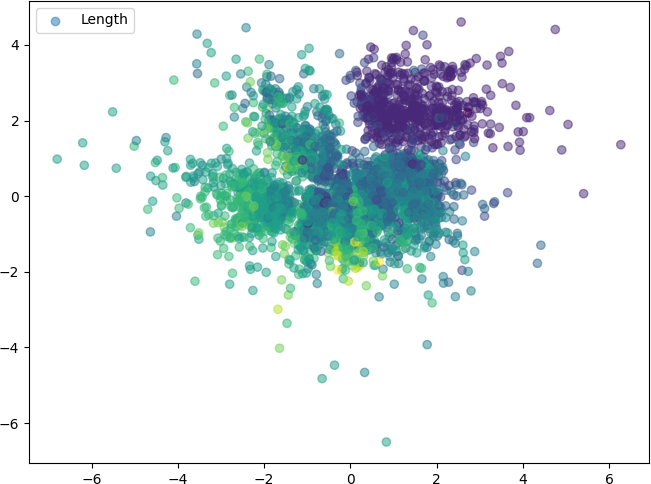
\includegraphics[width=\textwidth]{images/latent_spaces/mnist/vae/embeddings_mu_3.png}
        \caption{Latent space colored by digit length}
        \label{subfig:vae_mnist_latent_space_length}
    \end{subfigure}
    \hfill
    \begin{subfigure}{.24\textwidth}
        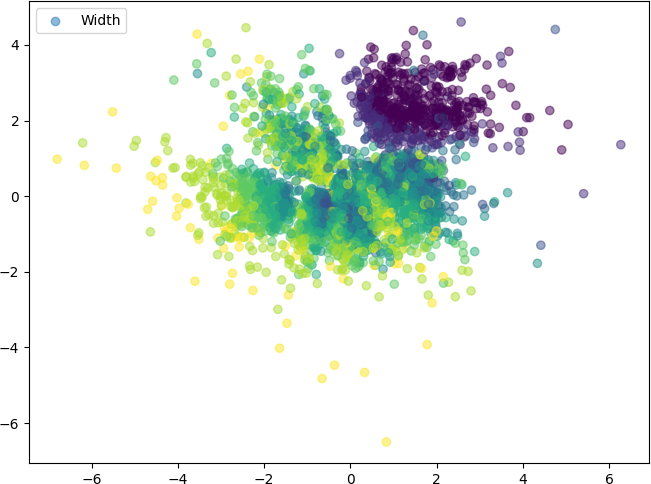
\includegraphics[width=\textwidth]{images/latent_spaces/mnist/vae/embeddings_mu_4.png}
        \caption{Latent space colored by digit width}
        \label{subfig:vae_mnist_latent_space_width}
    \end{subfigure}
    \hfill
    \begin{subfigure}{.24\textwidth}
        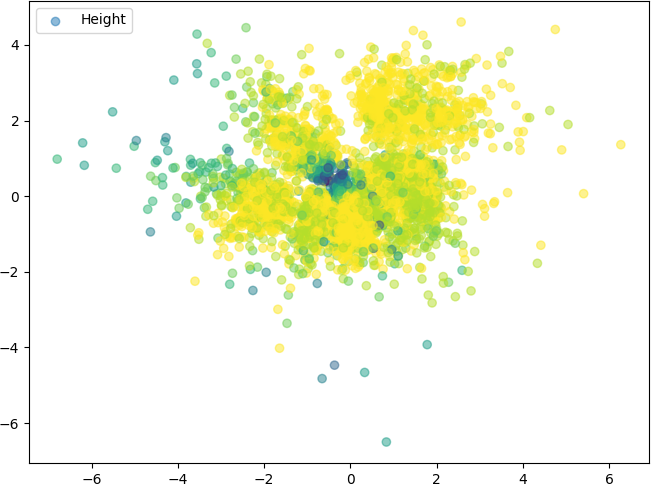
\includegraphics[width=\textwidth]{images/latent_spaces/mnist/vae/embeddings_mu_5.png}
        \caption{Latent space colored by digit height}
        \label{subfig:vae_mnist_latent_space_height}
    \end{subfigure}
    \hfill
    \begin{subfigure}{.24\textwidth}
        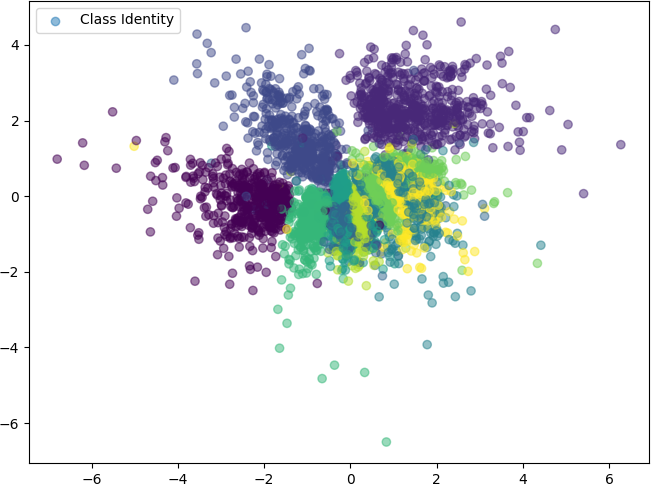
\includegraphics[width=\textwidth]{images/latent_spaces/mnist/vae/embeddings_mu_6.png}
        \caption{Latent space colored by digit identity}
        \label{subfig:vae_mnist_latent_space_identity}
    \end{subfigure}
    \caption[\ac{VAE} Latent Space on \textsc{Mnist}]{Latent space colored by different means of \ac{VAE} with $dim_z=2$ trained on \textsc{Mnist} dataset}
    \label{fig:vae_latent_space_mnist}
\end{figure}

\begin{landscape}
    \begin{figure}
        \centering
        \foreach \i in {1,2,3}{
        \begin{subfigure}{.16\textwidth}
            \includegraphics[width=\textwidth]{images/latent_spaces/mnist/vlae/embeddings_mu_\i_0.png}
            \caption{$z_{\i}$: digit slant}
            \label{subfig:vlae_mnist_latent_space_z_\i_slant}
        \end{subfigure}
        \hfill
        \begin{subfigure}{.16\textwidth}
            \includegraphics[width=\textwidth]{images/latent_spaces/mnist/vlae/embeddings_mu_\i_1.png}
            \caption{$z_{\i}$: digit thickness}
            \label{subfig:vlae_mnist_latent_space_z_\i_thickness}
        \end{subfigure}
        \hfill
        \begin{subfigure}{.16\textwidth}
            \includegraphics[width=\textwidth]{images/latent_spaces/mnist/vlae/embeddings_mu_\i_2.png}
            \caption{$z_{\i}$: digit area}
            \label{subfig:vlae_mnist_latent_space_z_\i_area}
        \end{subfigure}
        \hfill
        \begin{subfigure}{.16\textwidth}
            \includegraphics[width=\textwidth]{images/latent_spaces/mnist/vlae/embeddings_mu_\i_3.png}
            \caption{$z_{\i}$: digit length}
            \label{subfig:vlae_mnist_latent_space_z_\i_length}
        \end{subfigure}
        \hfill
        \begin{subfigure}{.16\textwidth}
            \includegraphics[width=\textwidth]{images/latent_spaces/mnist/vlae/embeddings_mu_\i_4.png}
            \caption{$z_{\i}$: digit width}
            \label{subfig:vlae_mnist_latent_space_z_\i_width}
        \end{subfigure}
        \hfill
        \begin{subfigure}{.16\textwidth}
            \includegraphics[width=\textwidth]{images/latent_spaces/mnist/vlae/embeddings_mu_\i_5.png}
            \caption{$z_{\i}$: digit height}
            \label{subfig:vlae_mnist_latent_space_z_\i_height}
        \end{subfigure}
        \hfill
        \begin{subfigure}{.16\textwidth}
            \includegraphics[width=\textwidth]{images/latent_spaces/mnist/vlae/embeddings_mu_\i_6.png}
            \caption{$z_{\i}$: digit identity}
            \label{subfig:vlae_mnist_latent_space_z_\i_identity}
        \end{subfigure}}
        \caption[\ac{VLAE} Latent Space on \textsc{Mnist}]{Latent space colored by different means of \ac{VLAE} with $dim_z=2$ trained on \textsc{Mnist} dataset}
        \label{fig:vlae_latent_space_mnist}
    \end{figure}
\end{landscape}

Noticeable, digit identity seems to be learned in $z_2$ as well as $z_3$ (see Figures~\ref{subfig:vlae_mnist_latent_space_z_2_identity} and \ref{subfig:vlae_mnist_latent_space_z_3_identity}).
This, however, would be a contradiction to Figure~\ref{subfig:vlae_mnist_latent_space_traversal} and even more Figure~\ref{subfig:vlae_gan_mnist_latent_space_traversal}, showing that digit identity mainly is learned in the last embedding layer.
Albeit $z_2$ has some influence on digit identity, this effect is not nearly as prominent as for $z_3$ even though the clustering in Figure~\ref{subfig:vlae_mnist_latent_space_z_2_identity} seems to be almost as good as in Figure~\ref{subfig:vlae_mnist_latent_space_z_3_identity}.
It seems as if the digit identity learned in $z_2$ only supports the model generation but has a far less strong influence than $z_3$.

All in all, \ac{VLAE} does not seem to learn fully separable representations.
However, the less powerful network below $z_1$ indeed seems to learn lower-level representations that also are employed when generating new images (see Figures~\ref{subfig:vlae_mnist_latent_space_traversal} and \ref{subfig:vlae_gan_mnist_latent_space_traversal}).

For \ac{VAE}, digit identity defines the shape of the latent space (Figure~\ref{subfig:vae_mnist_latent_space_identity}), leading to bigger \say{main clusters}.
As \ac{VAE} only has one latent space, it employs subspaces to learn the lower-level factors of variation such as slant within the main clusters (Figure~\ref{subfig:vae_mnist_latent_space_slant}).

The \ac{VAE} seems to learn an efficient encoding of most of the factors of variation as revealed by this kind of visualization even though it has narrower information bottleneck with a two-dimensional latent space compared to the three two-dimensional latent spaces of \ac{VLAE}.

\paragraph{CelebA}
\textbf{TODO}

\paragraph{dsprites}

The latent space embeddings for the dsprites dataset allow a more profound comparison of \ac{VAE} and \ac{VLAE}.
Here, the \ac{VAE} model was given a six-dimensional embedding space whereas the \ac{VLAE} model has three two-dimensional embedding spaces.
The dimensionality of the \ac{VAE} model was increased as the dsprites dataset was assumed to be more diverse compared to \textsc{Mnist}, requiring more model capacity to encode the information.
Importantly, \ac{VAE} and \ac{VLAE} approximately have the same model capacity under the assumption that \ac{VLAE} uses lower embedding layers to only learn lower-level features and higher embedding layers to only learn higher-level features and that the dataset can be splitted in this way.

As the \ac{VAE} model employs a higher dimensional latent space, the embeddings were visualized using t-SNE embeddings (see Figure~\ref{fig:vae_latent_space_dsprites}).

One advantage of dsprites over \textsc{Mnist} is that all factors of variation by design are independent and represented equally often, allowing a more straight-forward analysis.

\begin{figure}
    \centering
    \begin{subfigure}{.19\textwidth}
        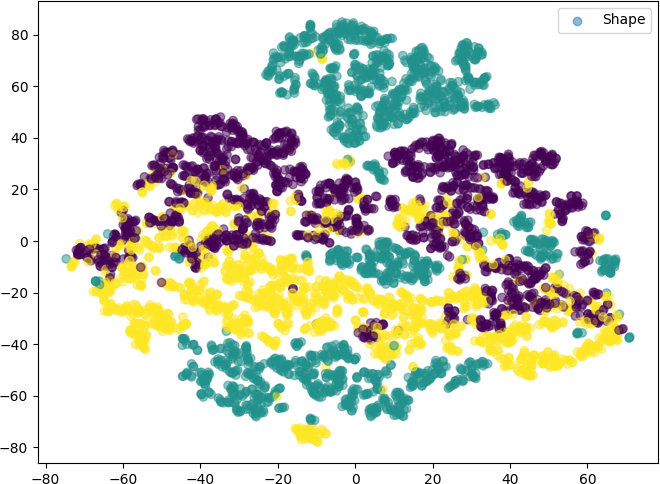
\includegraphics[width=\textwidth]{images/latent_spaces/dsprites/vae/embeddings_mu_0.png}
        \caption{Latent space colored by object shape}
    \end{subfigure}
    \hfill
    \begin{subfigure}{.19\textwidth}
        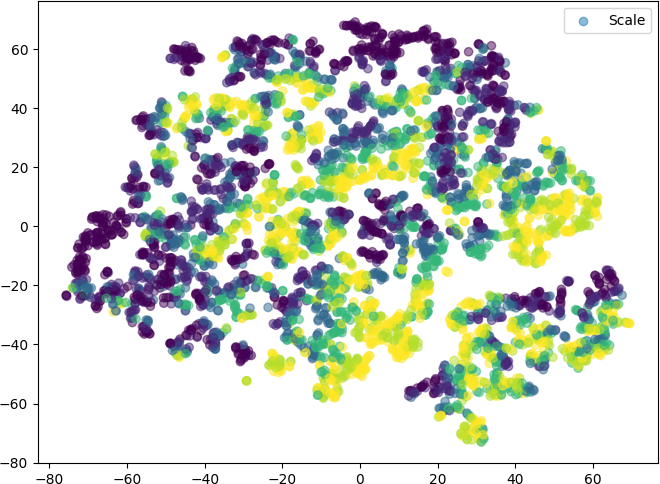
\includegraphics[width=\textwidth]{images/latent_spaces/dsprites/vae/embeddings_mu_1.png}
        \caption{Latent space colored by object scale}
        \label{subfig:vae_embedding_dsprites_scale}
    \end{subfigure}
    \hfill
    \begin{subfigure}{.19\textwidth}
        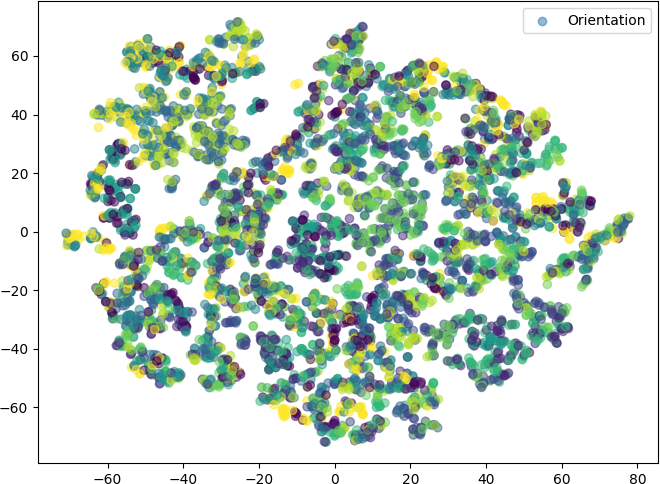
\includegraphics[width=\textwidth]{images/latent_spaces/dsprites/vae/embeddings_mu_2.png}
        \caption{Latent space colored by object orientation}
        \label{subfig:vae_embedding_dsprites_orientation}
    \end{subfigure}
    \hfill
    \begin{subfigure}{.19\textwidth}
        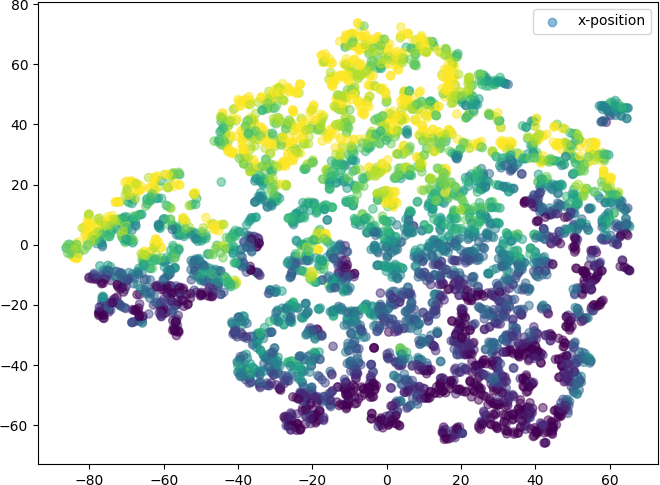
\includegraphics[width=\textwidth]{images/latent_spaces/dsprites/vae/embeddings_mu_3.png}
        \caption{Latent space colored by object $x$-position}
    \end{subfigure}
    \hfill
    \begin{subfigure}{.19\textwidth}
        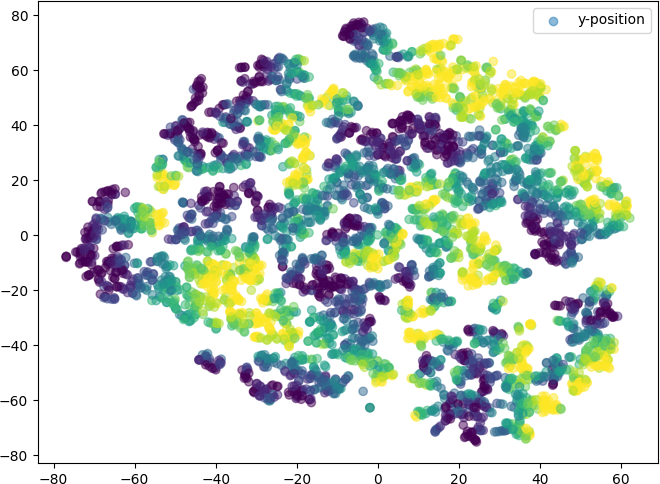
\includegraphics[width=\textwidth]{images/latent_spaces/dsprites/vae/embeddings_mu_4.png}
        \caption{Latent space colored by object $y$-position}
    \end{subfigure}
    \caption[\ac{VAE} Latent Space on dsprites]{t-SNE latent space embeddings colored by different means of \ac{VAE} with $dim_z=6$ trained on dsprites dataset}
    \label{fig:vae_latent_space_dsprites}
\end{figure}

\begin{figure}
    \centering
    \foreach \i in {1,2,3}{
    \begin{subfigure}{.19\textwidth}
        \includegraphics[width=\textwidth]{images/latent_spaces/dsprites/vlae/embeddings_mu_\i_0.png}
        \caption{Latent space $z_{\i}$ colored by object shape}
        \label{subfig:vlae_embedding_z\i_dsprites_shape}
    \end{subfigure}
    \hfill
    \begin{subfigure}{.19\textwidth}
        \includegraphics[width=\textwidth]{images/latent_spaces/dsprites/vlae/embeddings_mu_\i_1.png}
        \caption{Latent space $z_{\i}$ colored by object scale}
        \label{subfig:vlae_embedding_z\i_dsprites_scale}
    \end{subfigure}
    \hfill
    \begin{subfigure}{.19\textwidth}
        \includegraphics[width=\textwidth]{images/latent_spaces/dsprites/vlae/embeddings_mu_\i_2.png}
        \caption{Latent space $z_{\i}$ colored by object orientation}
        \label{subfig:vlae_embedding_z\i_dsprites_orientation}
    \end{subfigure}
    \hfill
    \begin{subfigure}{.19\textwidth}
        \includegraphics[width=\textwidth]{images/latent_spaces/dsprites/vlae/embeddings_mu_\i_3.png}
        \caption{Latent space $z_{\i}$ colored by object $x$-position}
        \label{subfig:vlae_embedding_z\i_dsprites_x_pos}
    \end{subfigure}
    \hfill
    \begin{subfigure}{.19\textwidth}
        \includegraphics[width=\textwidth]{images/latent_spaces/dsprites/vlae/embeddings_mu_\i_4.png}
        \caption{Latent space $z_{\i}$ colored by object $y$-position}
        \label{subfig:vlae_embedding_z\i_dsprites_y_pos}
    \end{subfigure}
    }
    \caption[\ac{VLAE} Latent Space on dsprites]{Latent space colored by different means of \ac{VLAE} with $dim_{z_i}=2$ trained on dsprites dataset}
    \label{fig:vlae_latent_space_dsprites}
\end{figure}

Again, the \ac{VAE} builds main clusters and seems to embed lower-level feature into main clusters.
Especially the object scale seems to be a lower-level feature (see Figure~\ref{subfig:vae_embedding_dsprites_scale}).
Only object orientation does not seem to be learned at all (see Figure~\ref{subfig:vae_embedding_dsprites_orientation}).

\ac{VLAE} performance on dsprites (see Figure~\ref{fig:vlae_latent_space_dsprites}) is worse compared to \ac{VAE}.
The model, again, learns main clusters, especially for object position (see Figures~\ref{subfig:vlae_embedding_z3_dsprites_x_pos} and \ref{subfig:vlae_embedding_z3_dsprites_y_pos}).
Furthermore, the model learns object scale (see Figure~\ref{subfig:vlae_embedding_z3_dsprites_scale} and \ref{subfig:vlae_embedding_z2_dsprites_scale}).
Otherwise, the model does not seem to learn other factors of variation.
Furthermore, the representations are not particularly disentangled.
Object position and scale is learned in all layers, but best in $z_3$.

All in all, using a \ac{VAE} with a higher-dimensional space seems to be superior compared to the \ac{VLAE} in terms of encoding effiency.

\subsubsection{Pixel-wise Image Statistics}\label{subsubsec:pixel_wise_statistics}

\acp{GAN} (see Section~\ref{subsubsec:representation_learning}) are trained by simulatenously training a \textit{generator} to create new samples and a \textit{discriminator} to discriminate between true and generated samples.
\acp{VAE} are another generative model that is not forced in the same way to create indistinguishable samples.
Instead, a reconstruction loss is used to force the reconstruction to be close to the true sample in terms of difference in the pixel values.
At the same time, the \ac{KL}-loss and the reparametrization trick force the model to place similar samples close toanother in a continuous Gaussian embedding space.
Drawing from the Gaussian embedding space therefore should allow to generate new samples similar to true samples.
However, the question remains how indistinguishable these generates samples are from true samples.

To address this question, different statistical analyses were performed revealing that in fact generated samples can be perfectly distinguished from true samples.

\paragraph{\textsc{Mnist}}

\begin{figure}
    \centering
    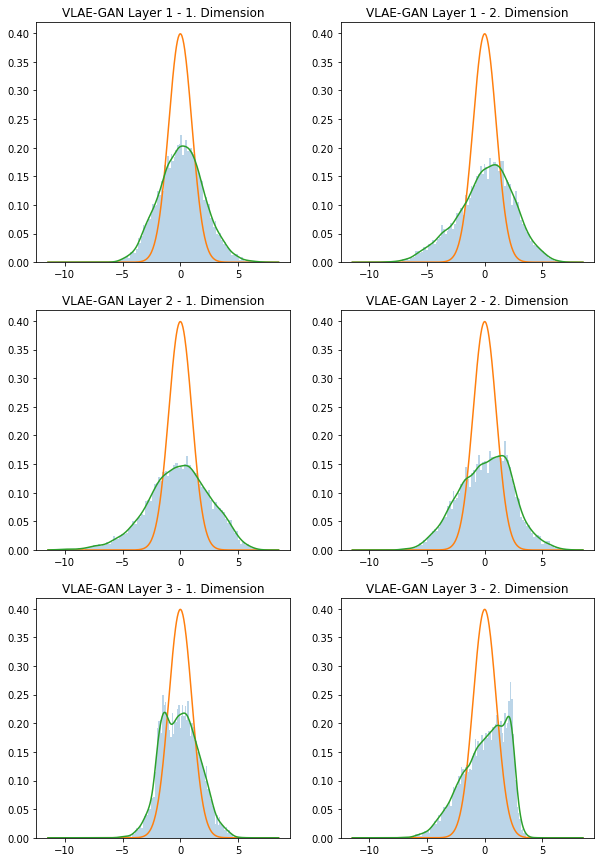
\includegraphics[width=.8\textwidth]{images/generated_vs_true/vlae_gan_kde.png}
    \caption[\ac{VLAE}-GAN - Latent Space Distribution]{Histogram of mean $z$-values for different layers and dimensions of \ac{VLAE}-\ac{GAN} (blue), the result of the \ac{KDE} (green), and a standard normal distribution (orange). Additional plots can be found in Appendix~\ref{sec:appendix_pixel_wise_statistics}.}
    \label{fig:vlae_gan_kde}
\end{figure}


\begin{figure}
    \centering
    \begin{subfigure}{0.48\textwidth}
        \centering
        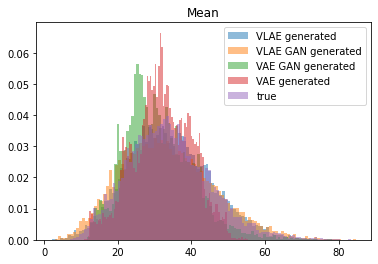
\includegraphics[width=\textwidth]{images/generated_vs_true/mnist_vs_models_mean.png}
        \caption{Histogram of mean pixel intensities for different models}
        \label{subfig:mean_generated_vs_true}
    \end{subfigure}
    \hfill
    \begin{subfigure}{0.48\textwidth}
        \centering
        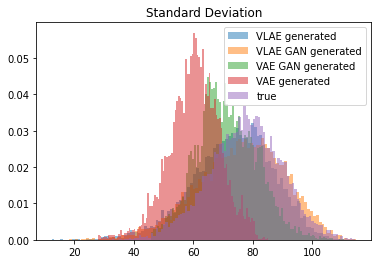
\includegraphics[width=\textwidth]{images/generated_vs_true/mnist_vs_models_sd.png}
        \caption{Histogram of pixel intensity standard deviations for different models}
        \label{subfig:sd_generated_vs_true}
    \end{subfigure}
    \hfill
    \begin{subfigure}{0.48\textwidth}
        \centering
        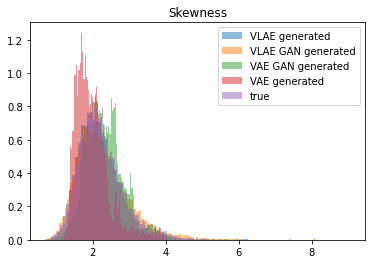
\includegraphics[width=\textwidth]{images/generated_vs_true/mnist_vs_models_skew.png}
        \caption{Histogram of pixel intensity skewness for different models}
        \label{subfig:skew_generated_vs_true}
    \end{subfigure}
    \hfill
    \begin{subfigure}{0.48\textwidth}
        \centering
        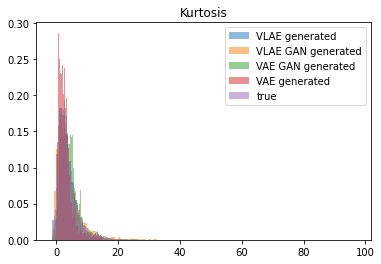
\includegraphics[width=\textwidth]{images/generated_vs_true/mnist_vs_models_kurt.png}
        \caption{Histogram of pixel intensity kurtosis for different models}
        \label{subfig:kurt_generated_vs_true}
    \end{subfigure}
    \caption[Models on \textsc{Mnist}: Pixel-wise distributions]{Pixel-wise distributions of different models and moments for the validation data set.}
    \label{fig:mean_generated_vs_true}
\end{figure}

The following procedure was applied to generate samples for different models.
One part of the \ac{VAE} loss function (and of the other models) is the \ac{KL}-term, forcing the models to match a standard multivariate normal distribution.
The learned distribution, however, is not perfectly Gaussian because of the other loss function terms.
Therefore, the model's encoders first predicted the mean values in $z$-space for the 10,000 validation images of the \textsc{Mnist} dataset.
Subsequently, for each dimension, \ac{KDE} was performed to estimate the \ac{PDF} of the latent space for \ac{VAE} and \ac{VAE}-\ac{GAN}.
Since the learned distribution by definition is covariance-free, the \ac{KDE} was performed for each dimension separately.
The estimated \ac{PDF} was then used to generate 1,000 new images to perform the statistical analyses on.
Figure~\ref{fig:vae_gan_kde} shows the estimated \ac{KDE} for \ac{VAE}-\ac{GAN}, plots for the other models can be found in Appendix~\ref{sec:appendix_pixel_wise_statistics}.

For \ac{VLAE} and \ac{VLAE}-\ac{GAN}, it cannot be sampled independently from the different latent spaces (see Section~\ref{subsec:independence-of-vlae-embeddings}).
For these models, the predicted mean values directly were used to reconstruct 10,000 images.

The MNIST test set of 10,000 images was compared to a 1,000 generated samples from \ac{VAE}, \ac{VLAE}, \ac{VAE}-\ac{GAN} and \ac{VLAE}-\ac{GAN}.
First, the mean pixel values, i.e.~the mean over all $28\times 28$ pixel values, were compared (see Figure~\ref{subfig:vlae_mean_generated_vs_true}).
The plot overlays the histograms of mean pixel values for the five conditions: \textsc{Mnist}, \ac{VAE}, and \ac{VLAE}.
The other plots in Figure~\ref{fig:mean_generated_vs_true} were created accordingly but for higher moments of the pixel value distributions.

Analyzing Figure~\ref{fig:mean_generated_vs_true} leads to the assumption that all models learn the pixel distributions to some extent.
The overlap of the histograms is high for all models.
\begin{table}
    \begin{tabular}{lrrrr}
        \toprule
        Model              & $p$-value (mean)    & $p$-value (sd)      & $p$-value (skewness) & $p$-value (kurtosis) \\
        \midrule
        \ac{VAE}           & $6.5\cdot 10^{-15}$ & 0.0                 & $3.7\cdot 10^{-257}$ & $1.4\cdot 10^{-70}$  \\
        \ac{VLAE}          & 0.439               & $4.1\cdot 10^{-98}$ & $1.1\cdot 10^{-8}$   & .0                   \\
        \ac{VAE}-\ac{GAN}  & $6.7\cdot 10^{-75}$ & 0.0                 & $9.3\cdot 10^{-48}$  & $2.2\cdot 10^{-63}$  \\
        \ac{VLAE}-\ac{GAN} & .0                  & $4.0\cdot 10^{-6}$  & 0.023                & 0.227                \\
        \bottomrule
    \end{tabular}
    \caption{$p$-values of a Mann-Whitney U test. Each cell tests the hypothesis that the respective moments for the respective model are equal to the values for the \textsc{MNIST} test images. For each cell, the sample size was $2\cdot 10,000$.}
    \label{tab:vae-vlae-mnist}
\end{table}
Table~\ref{tab:vae-vlae-mnist} shows the results of a two-sided Mann-Whitney $U$ test for the samples of moments of the pixel distributions.
The results lead to two conclusions: 1) The \ac{VLAE}-models capture the statistics of the pixel distribution better compared to the \ac{VAE}-models.
2) All models do not capture the true pixel distribution.

To verify that none of the models generates indistinguishable samples, a discriminator network was trained to distinguish generated samples from true \textsc{MNIST} test images\footnote{The configuration of the discriminator network can be found in Appendix~\ref{sec:listing_discriminator_network}. The network was trained using binary cross entropy for one epoch using the Adam optimizer.}.
The discriminator network shows an accuracy of 1.0 for distinguishing for all models, i.e.~it is perfectly able to predict generated from true samples for all models.

Comparing the pixel-wise statistics between generated (according to the \ac{KDE} procedure explained above) and reconstructed samples furthermore showed that there is a significant difference ($p < 0.001$, two-sided Mann-Whitney $U$ test) even though the difference between the $\bm{z}$ distribution of encoded validation images and $\bm{z}$s sampled from the estimated posterior is not significant ($p < 0.001$, two-sided Mann-Whitney $U$ test).
The reason for this is assumed to lie in samples for which the encoder predicts very low values $\log \sigma^2$ that have been observed during training.
Enforcing a lower bound for $\log \sigma^2$ in the encoder could prevent this.

\paragraph{CelebA}
\textbf{TODO: Plots and Discussion}

\paragraph{dsprites}
\textbf{TODO: Plots and Discussion}

\subsubsection{Distribution of Generated Samples}

Do the \ac{VAE} and \ac{VLAE} models generate each number with the same probability as a number's probability in the training set?
To answer this question, the following procedure was applied.

First, let each model generate a large number of images by drawing the latent space variable(s) $z$ from their estimated posterior (see Section~\ref{subsubsec:pixel_wise_statistics} for details).
Second, let a classifier\footnote{The classifier has shown to perform sufficiently well, see above.} classify each generated image.

This procedure was applied to \textsc{Mnist} only as it was the only labeled dataset where the \acp{VAE} and \acp{VLAE} models have shown a promising performance and for the availability of labels.

\begin{figure}
    \centering
    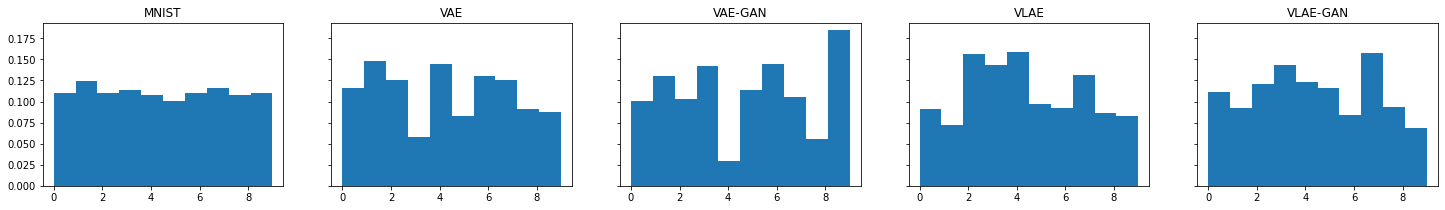
\includegraphics[width=\textwidth]{images/generated_vs_true/class_distr.png}
    \caption{Distribution of generated class labels for different models.}
    \label{fig:generated_class_distribution}
\end{figure}

Figure~\ref{fig:generated_class_distribution} shows the class-distribution of generated images.
Even though it is sampled from the true (estimated) posterior, the class distribution is quite uneven.
This aligns with Figure~\ref{fig:mnist_latent_space_traversal}.
The reason why the models maps some digits to very small subspaces, however, remains unclear.
If it was because there is less variation for a certain digit, i.e.~the digit three is written very similar in all cases, then all models should map threes to small subspaces.

However, \ac{VAE} reproduces few threes wheres \ac{VAE}-\ac{GAN} produces few fours.

Overall, the \ac{VLAE} models generate a more even distribution of generated digits.

\begin{figure}
    \centering
    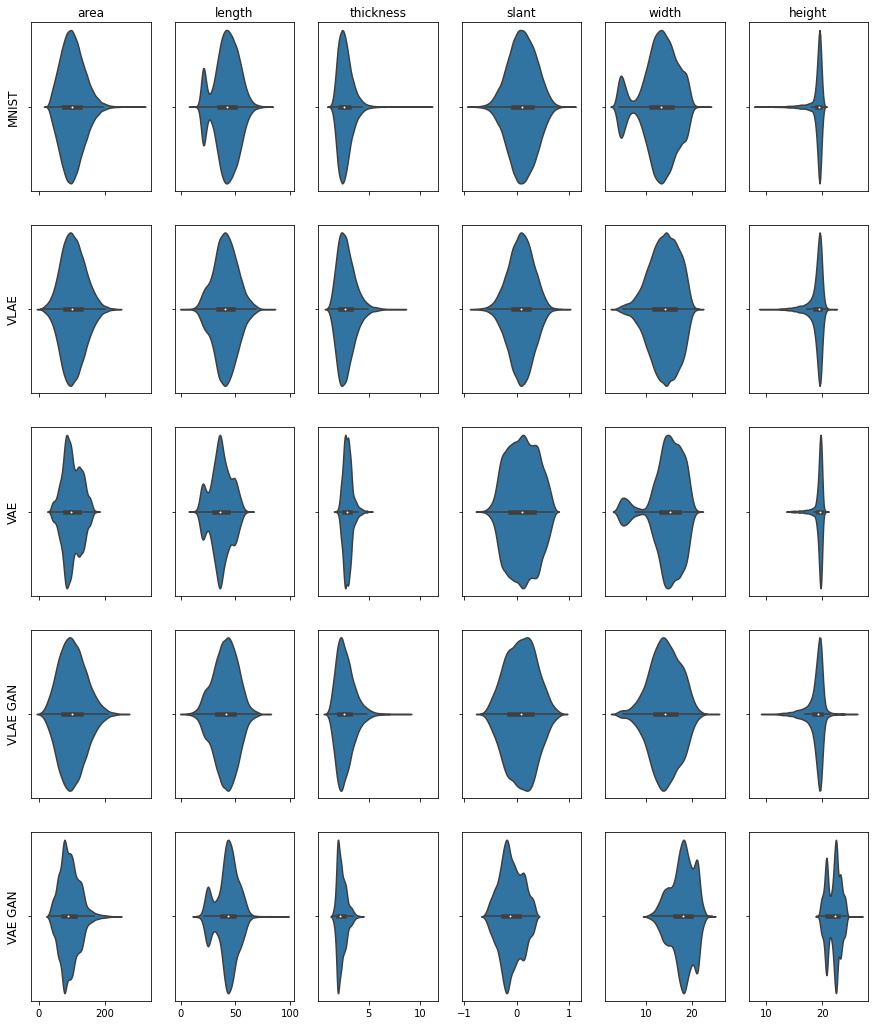
\includegraphics[width=\textwidth]{images/generated_vs_true/morpho_distr.png}
    \caption{Distribution of Morpho- \textsc{Mnist} attributes for different models.}
    \label{fig:generated_morpho_distribution}
\end{figure}

Figure~\ref{fig:generated_morpho_distribution} shows the distribution of morphological attributes for generated digits.
The Figure is accordingly to Figure~\ref{fig:morpho_mnist_distribution}.
The bottom row in Figure~\ref{fig:morpho_mnist_distribution} is equivalent to the top row in Figure~\ref{fig:generated_morpho_distribution}.

The \ac{VLAE} models learn a smooth distribution for most attributes that approximately resembles the true distribution.
They fail, however, in generating the same proportion of digits with a small width (i.e. the digit \textit{one}).
The \ac{VAE} model (but not \ac{VAE}-\ac{GAN}) is more successful in that regard.
However, the \ac{VAE} distributions are less smooth compared to the \ac{VLAE} models.

\textbf{Discuss Figure~\ref{fig:generated_morpho_distribution}}

\subsubsection{Independence of VLAE Embeddings}\label{subsec:independence-of-vlae-embeddings}

The VLAE learns embeddings on different levels.
For MNIST, \citet{zhao2017learning} used three two-dimensional layers to learn image semantics of different granularity.
They claim that their model is able to learn disentangled hierarchical features.
Figure~\ref{subfig:vlae_mnist_latent_space_traversal} shows reconstructions of this model when systematically exploring one dimensions and randomly choosing the others.
Apparently, the model is able to learn disentangled representations to some extent.

For example, $z_1$ seems to mainly encode the digit thickness whereas $z_3$ seems to encode digit identity.
For $z_2$, however, seems to also have influence on the digit identity.
Therefore, it is not obvious how disentangled the representations actually are.
\begin{breakablealgorithm}
    \caption{Generating Layer Representative Samples by Averaging Out Other Embedding Layers}\label{alg:layer_representative_samples}
    \begin{algorithmic}[1]
        \Function{LayerRepresentativeSamples}{numSamples,numApproximations}
            \State $j \gets 0$
            \State $\mathcal{L}\gets \varnothing$
            \While{$i < \text{numSamples}$}
                \State $\bm{v} \gets \bm{v} \sim \mathcal{N}(\bm{0}, \bm{I})$\label{line:fixing_v}
                \ForAll{$j \in \{1,2,3\}$}
                    \State $\bm{s}_j \gets$ \Call{LayerRepresentativeSample}{$\bm{v}$, numApproximations, $j$}
        \EndFor
        \State $\mathcal{L} \gets \mathcal{L} \cup \{\{\bm{s}_1, \bm{s}_2, \bm{s}_3\}\}$

        \EndWhile
        \State \Return $\mathcal{L}$
        \EndFunction

        \Function{LayerRepresentativeSample}{fixedDimensionValue, numApproximations, dimensionIndex}
        \State $\mathcal{D} \gets \{1,2,3\}$
        \State $\alpha \gets \text{fixedDimensionValue}$
        \State $\beta \gets (D \setminus \text{dimensionIndex})_1$
        \State $\gamma \gets (D \setminus \text{dimensionIndex})_2$
        \State $\bm{z}_{\alpha} \gets \bm{a} \sim \mathcal{N}(\bm{0}, \bm{I})$
        \State $\mathcal{L}\gets \varnothing$
        \State $i \gets 0$
        \While{$i < \text{numApproximations}$}
        \State $\bm{z}_{\beta}^i \gets \bm{b}_i \sim \mathcal{N}(\bm{0}, \bm{I})$
        \State $\bm{z}_{\gamma}^i \gets \bm{c}_i \sim \mathcal{N}(\bm{0}, \bm{I})$
        \State $\mathcal{L} \gets \mathcal{L} \cup \{$ \Call{VLAE-Decoder}{$\bm{z}_{\alpha}, \bm{z}_{\beta}^j, \bm{z}_{\gamma}^j$} $\}$
        \State $i \gets i + 1$
        \EndWhile
        \State \Return $\frac{1}{|\mathcal{L}|}\sum_j \mathcal{L}_j$
        \EndFunction
    \end{algorithmic}
\end{breakablealgorithm}

Consider Algorithm~\ref{alg:layer_representative_samples}.
The function \textsc{VLAE-Decoder} calls the decoder of the VLAE, i.e. $p_\theta(\bm{x} | \bm{z}_1, \bm{z}_2, \bm{z}_3)$.
Calling the function \textsc{LayerRepresentativeSamples} returns an ordered set $\mathcal{L}$ of \say{layer representative samples}.
Each sample $i$ contains three items, say $\bm{x}_1^i, \bm{x}_2^i, \bm{x}_3^i$ that were created by fixing a value $\bm{v}$ in Line~\ref{line:fixing_v} of Algorithm \ref{alg:layer_representative_samples}.
What is meant by the term \say{layer representative samples} is that for example $\bm{x}_1^i$ is approximately drawn from the marginal distribution
\begin{align}
    \bm{x}_1^i \sim p_\theta(\bm{v} | \bm{z}_1) = \int_{\bm{z}_2} \int_{\bm{z}_3} p_\theta(\bm{v} | \bm{z}_1, \bm{z}_2, \bm{z}_3) d\bm{z}_2 d\bm{z}_3
\end{align}
Now, if the embedding layers learn disentangled hierarchical representations, $p_\theta(\bm{x} | \bm{z}_1)$, $p_\theta(\bm{x} | \bm{z}_2)$, and $p_\theta(\bm{x} | \bm{z}_3)$ should be pairwise statistically independent.
Specifically,
\begin{align}
    p_\theta(\bm{x} | \bm{z}_i) \not \propto p_\theta(\bm{x} | \bm{z}_j) \quad \forall (i,j):i\neq j \label{eq:notprop}
\end{align}

However, this is not true.
Choosing a value $\bm{z}_1 = \varphi$ such that $p_\theta(\bm{x} | \bm{z}_1 = \varphi)$ also leads to a high value of $p_\theta(\bm{x} | \bm{z}_2 = \varphi)$, leading to a violation of Equation \ref{eq:notprop}.

\begin{figure}
    \centering
    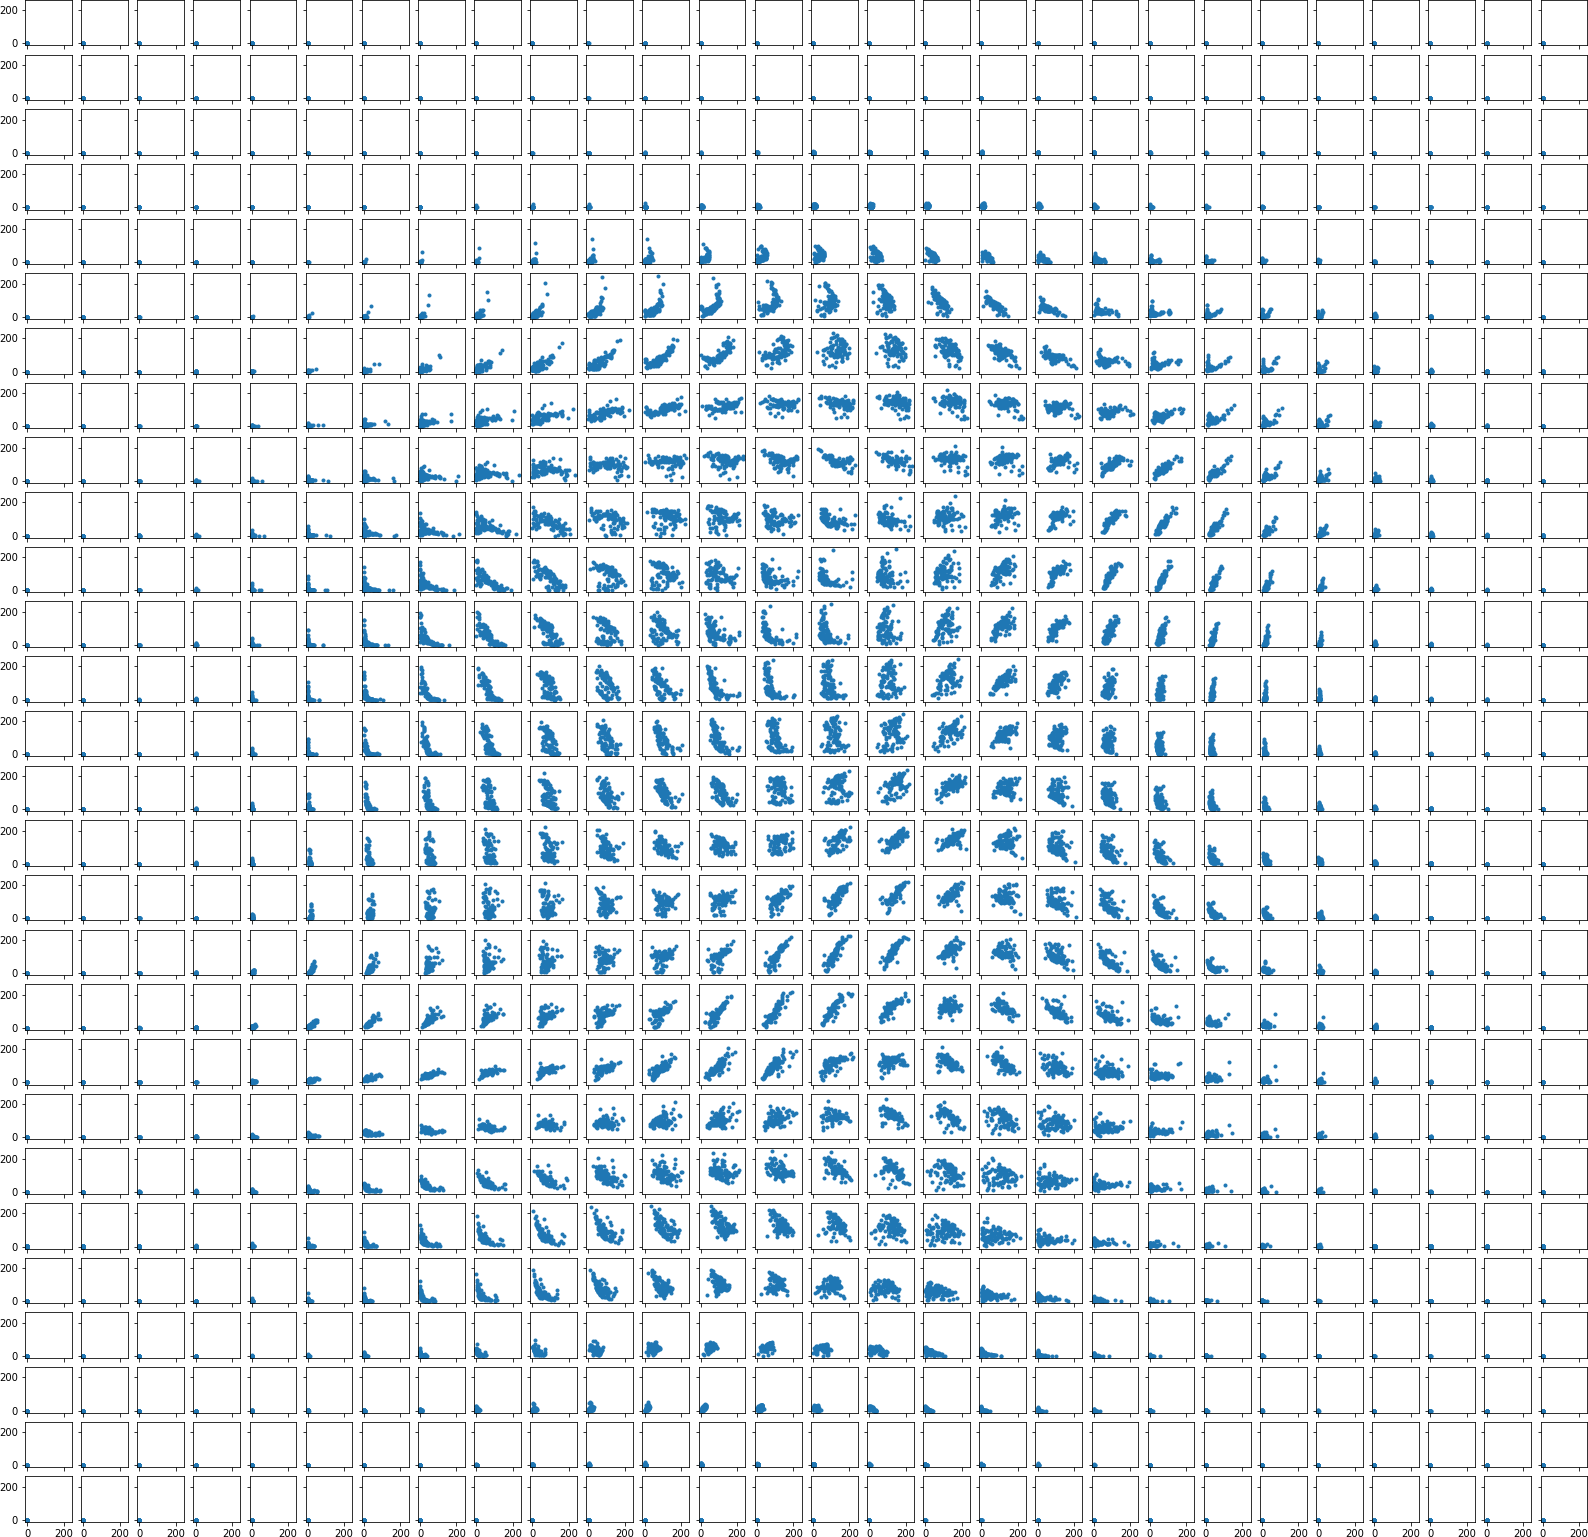
\includegraphics[width=\textwidth]{images/notprop/mnist/vlae/ccs_0_1_vlae.png}
    \caption[\ac{VLAE} on \textsc{Mnist} - Pixel proportionality]{Proportionality of pixel intensities when fixing $\bm{z}_1 = \bm{z}_2=\varphi$ for \ac{VLAE} trained on \textsc{Mnist}. Each box represents one of $28\times 28$ MNIST pixels. The $x$-axis of each box encodes the mean pixel intensity of the $\bm{z}_1$-representative sample. The $y$-axis encodes the mean pixel intensity of the of the $\bm{z}_2$-representative sample. Dots within boxes belong to the same $\varphi$ for both, $\bm{z}_1$ and $\bm{z}_2$. }
    \label{fig:notprop}
\end{figure}

Consider Figure~\ref{fig:notprop}.
It shows results of samples $(\bm{x}_1^1,\bm{x}_2^1),\dots,(\bm{x}_1^{100},\bm{x}_{100}00)$ that were generated by Algorithm~\ref{alg:layer_representative_samples}.
Thus, the parameter \say{numSamples} is chosen as 100 and the parameter \say{numApproximations} is chosen as 300.
Each $\bm{x}_i^j$ is one generated MNIST image of size $28\times 28$ pixels.
Each box in Figure~\ref{fig:notprop} corresponds to one of these pixels, the box index corresponds to the pixel in the MNIST image.
The $x$-values of dots in the same box then correspond to $\bm{x}_1^1\big|_{(3,1)}, \dots, \bm{x}_1^{100}\big|_{(3,1)}$, i.e. the pixel intensities of one specific pixel (here: third row, first column (3,1)) over all 100 samples for $\bm{x}_1$, i.e. the sample generated by fixing $\bm{z}_1$.
Analogously, the $y$-values of dots in the same box correspond to $\bm{x}_2^1\big|_{(3,1)}, \dots, \bm{x}_2^{100}\big|_{(3,1)}$.
Each dot corresponds to one fixed $\varphi$-value.

Now, if changing the value of $\bm{z}_1$ was independent of changing the value of $\bm{z}_2$, the boxes should show now trend.
This is true for outer boxes.
They correspond to pixel values that always close to zero, therefore the value are in the bottom left corner and no correlation can be observed.
For center pixels, however, the plot shows something different.
They show an interesting correlation pattern of negative and positive correlations.

Negative correlations for a pixel with index $(i,j)$ indicate that $p_\theta(\bm{x}\big|_{(i,j)} | \bm{z}_1 = \varphi) \propto \frac{1}{p_\theta(\bm{x}\big|_{(i,j)} | \bm{z}_1 = \varphi)}$, i.e. choosing a value $\varphi$ that leads to a high $(i,j)$-pixel intensity for the $\bm{z}_1$-representative sample leads to a low intensity of the same pixel of the corresponding $\bm{z}_1$-representative sample.
This, however, is a violation of equation~\ref{eq:notprop}.
Importantly, the correlation only persists for certain pixels.

The qualitative behavior is similar for all \ac{VLAE} models.
All plots can be found in Appendix~\ref{sec:additional-plots-for-section_independence}.

\subsubsection{CelebA}

\textbf{TODO}

\subsection{Latent Space Entanglement and Categorical Factors of Variation}\label{subsec:latent-space-entanglement-and-categorical-factors-of-variation}

As discussed in Section~\ref{subsec:feature-disentanglement} and Section~\ref{subsubsec:representation_learning} ($\beta$-\ac{VAE}), there is a trade-off between reconstruction quality and prior-posterior matching.
Increasing the weight of the reconstruction term in the \ac{VAE} training objective (smaller $\beta$ in Equation~\ref{eq:beta-vae}) leads to better reconstructions.
The posterior distribution, however, will match the prior distribution less exactly.
Increasing $\beta$ in Equation~\ref{eq:beta-vae}, in contrast, leads to a posterior closer to the prior distribution at the expense of reconstruction quality.

Specifically, \citet{higgins2017beta} claim that increasing $\beta$ leads to a better latent space disentanglement.

As discussed in Section~\ref{subsec:feature-disentanglement}, the quality of feature space disentanglement can be assessed by measuring how fast reconstructions change as the latent space is traversed.
A well disentangled feature space, however, should lead to problems for datasets with categorical factors of variation such as dsprites.
Even though CelebA has binary labels as well (for example \say{brown hair}), there still is enough variation within hair colors to allow a smooth translation between hair colors~\citep{higgins2017beta}.
For dsprites, there are only three distinct shapes (\say{square}, \say{ellipse}, and \say{heart}).
To achieve a good reconstruction quality on these shapes, the model would have to place them in separate areas of the latent space, violating both, feature space disentanglement and a Gaussian posterior.

To validate this empirically, a \ac{VAE} with input size $64\times 64$ (the size of dsprites images) and a ten-dimensional latent space was trained on dsprites with different reconstruction term weights: 10,000, 7,500, and 5,000.
For the remainder of this section, these models are referred to as \say{10,000-\ac{VAE}}, \say{7,500-\ac{VAE}}, and \say{\say{5,000-\ac{VAE}}}.

\begin{figure}
    \centering
    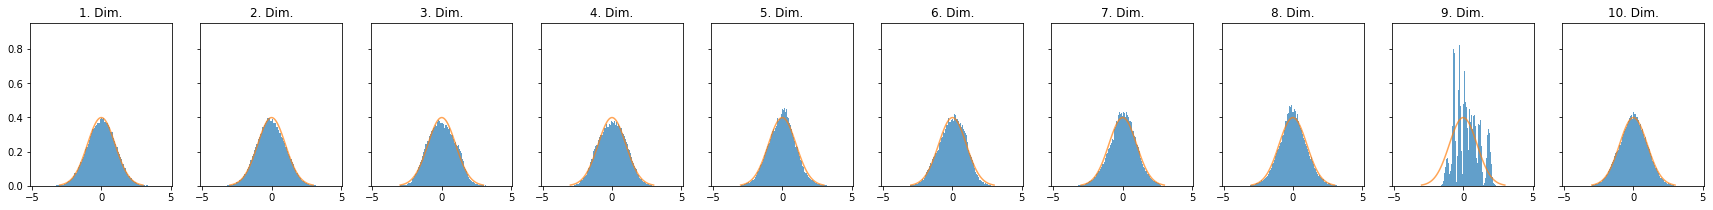
\includegraphics[width=\textwidth]{images/latent_space_entanglement/vae_dsprites_lf_10000_dist.png}
    \caption{Histogram of 73,728 dsprites images from the validation set in 100 bins for \ac{VAE} with reconstruction term weight 10,000}
    \label{fig:10000_vae_latent_space_distribution}
\end{figure}

Figure~\ref{fig:10000_vae_latent_space_distribution} shows the distribution of dsprites validation images.
Noticeable, the ninth dimension is far less Gaussian than the other nine dimensions.
As \say{object shape} is the only categorical factor of variation, one could assume that the ninth dimension encodes \say{object shape}.
However, this raises the question why there are more than three peaks for the ninth dimension.

\begin{figure}
    \centering
    \begin{subfigure}{\textwidth}
        \centering
        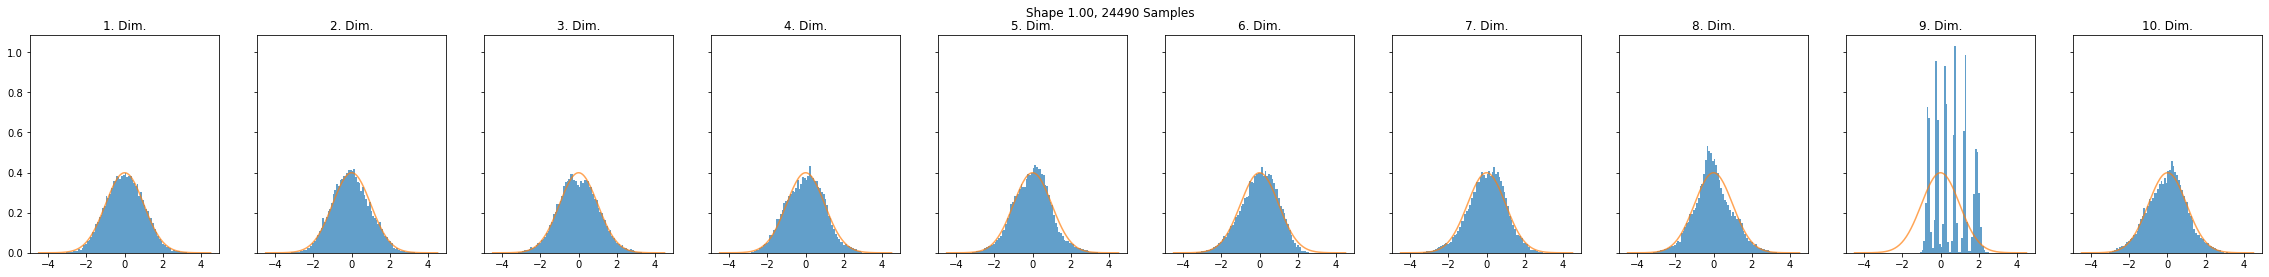
\includegraphics[width=\textwidth]{images/latent_space_entanglement/vae_dsprites_lf_10000_dist_shape_1.png}
        \caption{Latent space distribution of images with shape \textit{Square}}
    \end{subfigure}
    \begin{subfigure}{\textwidth}
        \centering
        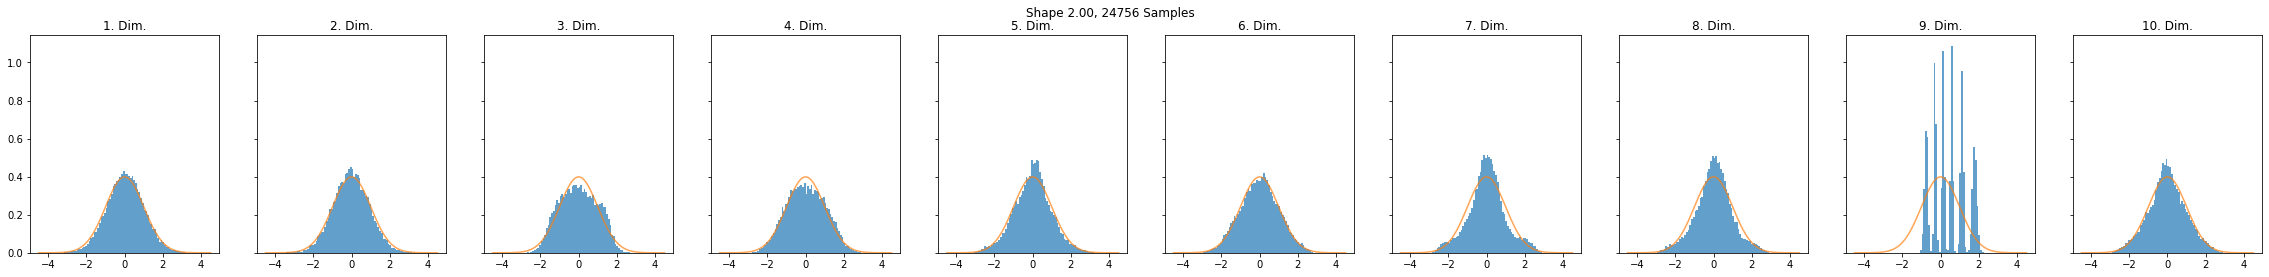
\includegraphics[width=\textwidth]{images/latent_space_entanglement/vae_dsprites_lf_10000_dist_shape_2.png}
        \caption{Latent space distribution of images with shape \textit{Ellipse}}
    \end{subfigure}
    \begin{subfigure}{\textwidth}
        \centering
        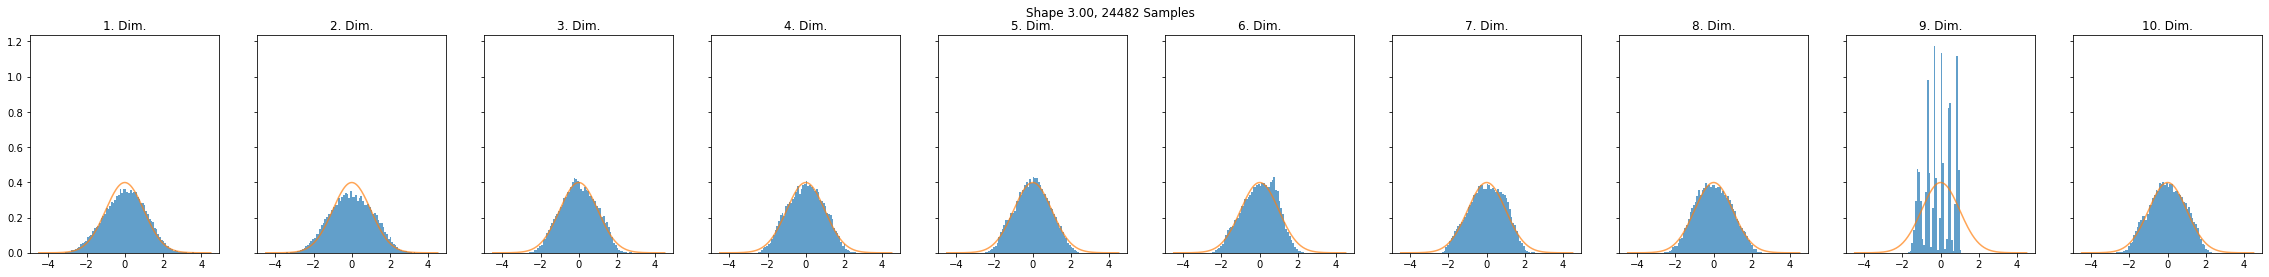
\includegraphics[width=\textwidth]{images/latent_space_entanglement/vae_dsprites_lf_10000_dist_shape_3.png}
        \caption{Latent space distribution of images with shape \textit{Heart}}
    \end{subfigure}
    \caption{Histogram of dsprites images with a certain shape from the validation set in 100 bins}
    \label{fig:10000_vae_latent_space_distribution_shapes}
\end{figure}

Figure~\ref{fig:10000_vae_latent_space_distribution_shapes} shows the distribution of images with a certain shape.
Even though there is some difference between the plots, the $\mu$-values in the ninth dimension still are assigned to different and distinct areas within the ninth dimension.
\textit{Shape} alone does not explain the strong peaks in the ninth dimension.

\begin{figure}
    \centering
    \begin{subfigure}{\textwidth}
        \centering
        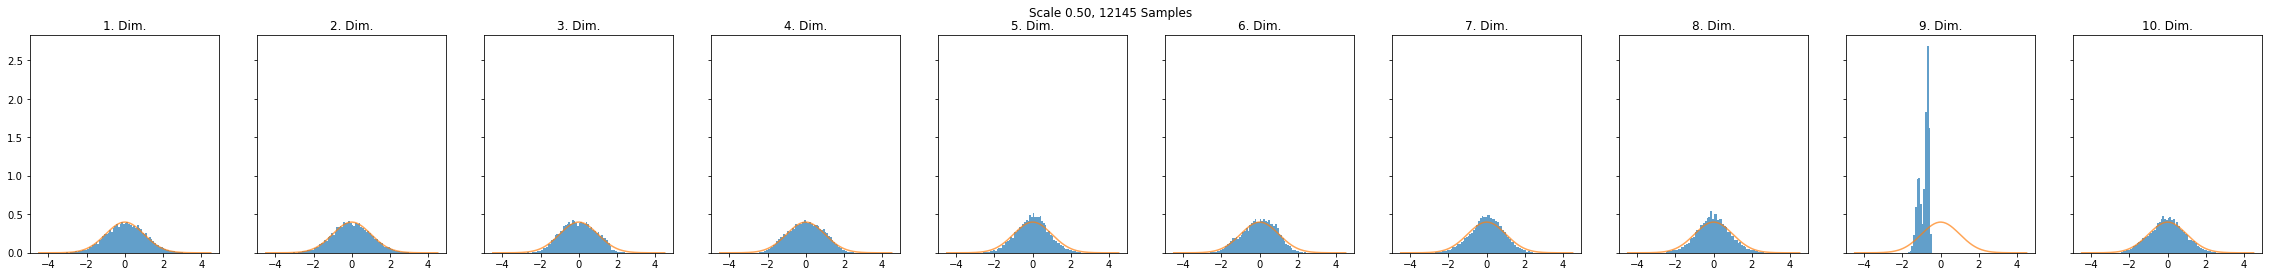
\includegraphics[width=\textwidth]{images/latent_space_entanglement/vae_dsprites_lf_10000_dist_scale_0_5.png}
        \caption{Latent space distribution of images with scale = 0.5}
    \end{subfigure}
    \begin{subfigure}{\textwidth}
        \centering
        \includegraphics[width=\textwidth]{images/latent_space_entanglement/vae_dsprites_lf_10000_dist_scale_0_6.png}
        \caption{Latent space distribution of images with scale = 0.6}
    \end{subfigure}
    \begin{subfigure}{\textwidth}
        \centering
        \includegraphics[width=\textwidth]{images/latent_space_entanglement/vae_dsprites_lf_10000_dist_scale_0_7.png}
        \caption{Latent space distribution of images with scale = 0.7}
    \end{subfigure}
    \begin{subfigure}{\textwidth}
        \centering
        \includegraphics[width=\textwidth]{images/latent_space_entanglement/vae_dsprites_lf_10000_dist_scale_0_8.png}
        \caption{Latent space distribution of images with scale = 0.8}
    \end{subfigure}
    \begin{subfigure}{\textwidth}
        \centering
        \includegraphics[width=\textwidth]{images/latent_space_entanglement/vae_dsprites_lf_10000_dist_scale_0_9.png}
        \caption{Latent space distribution of images with shape scale = 0.9}
    \end{subfigure}
    \begin{subfigure}{\textwidth}
        \centering
        \includegraphics[width=\textwidth]{images/latent_space_entanglement/vae_dsprites_lf_10000_dist_scale_1_0.png}
        \caption{Latent space distribution of images with shape scale = 1.0}
    \end{subfigure}
    \caption{Histogram of dsprites images with a certain scale from the validation set in 100 bins}
    \label{fig:10000_vae_latent_space_distribution_scales}
\end{figure}

Consider Figure~\ref{fig:10000_vae_latent_space_distribution_scales} showing distributions of images of differenct \textit{scales}.
The scale values in the dsprites dataset are six distinct values in the range from 0.5 to 1.0.
Apparently, a \ac{VAE} model with a too strong reconstruction term does not learn to interpolate between these values but assigns them to distinct areas of the latent space.

Plotting only the images with a certain scale \textit{and} a certain shape, finally, explains the distinct peaks in the ninth dimension (see Figure~\ref{fig:10000_vae_latent_space_distribution_scales_and_shapes}).
The model produces two peaks for each scale.
One of the peaks attributes to the shape \textit{Heart}, the other one for the shapes \textit{Ellipse} and \textit{Square}.

\begin{figure}
    \centering
    \begin{subfigure}{\textwidth}
        \centering
        \includegraphics[width=\textwidth]{images/latent_space_entanglement/vae_dsprites_lf_10000_dist_shape_1_scale_0_5.png}
        \caption{Latent space distribution of images with scale = 0.5 and shape \textit{Square}}
    \end{subfigure}
    \begin{subfigure}{\textwidth}
        \centering
        \includegraphics[width=\textwidth]{images/latent_space_entanglement/vae_dsprites_lf_10000_dist_shape_2_scale_0_5.png}
        \caption{Latent space distribution of images with scale = 0.5 and shape \textit{Ellipse}}
    \end{subfigure}
    \begin{subfigure}{\textwidth}
        \centering
        \includegraphics[width=\textwidth]{images/latent_space_entanglement/vae_dsprites_lf_10000_dist_shape_3_scale_0_5.png}
        \caption{Latent space distribution of images with scale = 0.5 and shape \textit{Heart}}
    \end{subfigure}
    \caption{Histogram of dsprites images with scale = 0.5 and different shapes from the validation set in 100 bins}
    \label{fig:10000_vae_latent_space_distribution_scales_and_shapes}
\end{figure}

Noteworthy, the model learns a hierarchical clustering in the ninth dimension.
\textit{Shape} is a subcluster of \textit{Scale}.
Certainly, this subclustering leads to highly entangled latent space and a highly un-Gaussian distribution.
It allows, however, to violate the \textit{KL}-term in favor of the reconstruction term in just one instead of two dimensions.

\begin{figure}
    \centering
    \begin{subfigure}{\textwidth}
        \centering
        \includegraphics[width=\textwidth]{images/latent_space_entanglement/vae_10000_traverse_square_ellipse.png}
        \caption{Latent space traversal from \textit{Square} $\rightarrow$ \textit{Ellipse}}
        \label{subfig:10000_vae_latent_space_traversal_square_to_ellipse}
    \end{subfigure}
    \begin{subfigure}{\textwidth}
        \centering
        \includegraphics[width=\textwidth]{images/latent_space_entanglement/vae_10000_traverse_ellipse_heart.png}
        \caption{Latent space traversal from \textit{Ellipse} $\rightarrow$ \textit{Heart}}
    \end{subfigure}
    \begin{subfigure}{\textwidth}
        \centering
        \includegraphics[width=\textwidth]{images/latent_space_entanglement/vae_10000_traverse_heart_square.png}
        \caption{Latent space traversal from \textit{Heart} $\rightarrow$ \textit{Square}}
        \label{subfig:10000_vae_latent_space_traversal_heart_to_square}
    \end{subfigure}
    \caption{Latent space traversal between latent space representations of images with certain shapes for 10,000-\ac{VAE}. Color-values were inverted for this plot.}
    \label{fig:10000_vae_latent_space_traversal_shape_to_shape}
\end{figure}

Figure~\ref{fig:10000_vae_latent_space_traversal_shape_to_shape} shows the latent space traversal between different shapes\footnote{The corresponding plots for the other model can be found in Appendix~\ref{sec:additional_plots_latent_space_entanglement}.}.
For the purpose of the plot, the latent representations $\bm{z}_1, \bm{z}_2$ of two $\bm{x}_i$ with a certain shape and the same configuration of the other parameters was obtained and interpolated between linearly.
Figure~\ref{fig:10000_vae_latent_space_traversal_shape_to_shape} shows the reconstructions of 21 evenly spaced points on the line segment between $\bm{z}_1$ and $\bm{z}_2$.
It shows the high degree of latent space entanglement: sudden position changes (Figure~\ref{subfig:10000_vae_latent_space_traversal_square_to_ellipse}) or sudden emergence of new objects (Figure~\ref{fig:10000_vae_latent_space_traversal_shape_to_shape}).

Importantly, obtaining $\bm{z}$ by fixing only the shape and the scale\footnote{Based on the cluster analysis, not fixing the scale would easily lead to regions with low probability density.} for an $\bm{x}_i$ and averaging over all other configurations was not successful.
It lead to empty images as it probably lead to $\bm{z}_i$'s in regions of the latent space with low probability density.
Furthermore, for the latent space traversal shown in Figure~\ref{fig:10000_vae_latent_space_traversal_shape_to_shape}, it was possible to always find parameter combinations where the traversal lead to empty images in the middle of the line segment.

\begin{figure}
    \centering
    \begin{subfigure}{\textwidth}
        \centering
        \includegraphics[width=\textwidth]{images/latent_space_entanglement/vae_dsprites_lf_7500_dist.png}
        \caption{Reconstruction term weight 7,500}
    \end{subfigure}
    \begin{subfigure}{\textwidth}
        \centering
        \includegraphics[width=\textwidth]{images/latent_space_entanglement/vae_dsprites_lf_5000_dist.png}
        \caption{Reconstruction term weight 5,000}
    \end{subfigure}
    \caption{Histogram of 73,728 dsprites images from the validation set in 100 bins for \ac{VAE} with different reconstruction term weights}
    \label{fig:7500_5000_vae_latent_space_distribution_scales_and_shapes}
\end{figure}

Figure~\ref{fig:7500_5000_vae_latent_space_distribution_scales_and_shapes} shows the latent space distribution of \acp{VAE} with a reduced reconstruction term weight, i.e. an increase \ac{KL-divergence} term weight.
The histograms look more Gaussian and in fact the \ac{KL-divergence} on the validation set decreased from 22.744 (reconstruction loss weight: 10,000) to 22.271 (reconstruction loss weight: 7,500) or, respectively, 18.172 (reconstruction loss weight: 5,000).
Surprisingly, the difference between 10,000-\ac{VAE} and 7,500-\ac{VAE} is small on the validation data.

To account for latent space disentanglement, the \ac{PPL} for the latent spaces of the different models is computed.
The perceptual loss is obtained by a \ac{CNN} trained to predict dsprites object categories\footnote{The model architecture can be found in Appendix~\ref{sec:appendix_feature_extraction_network_ppl_dsprites}, the features are extracted in \say{conv2d\_94}. The model was trained for one epoch using categorical crossentropy with the Adam optimizer with an initial learning rate of 0.1. The model achieved a top-1 accuracy of 0.8 on the validation set.}.
The \ac{PPL} was computed for 50 different random seeds.
Each of these \ac{PPL}-computations interpolated at random 100 steps (dependent on the random seed).

\begin{table}
    \centering
    \begin{tabular}{lrr}
        \toprule
        Model           & mean \ac{PPL} & standard deviation \\
        \midrule
        10,000-\ac{VAE} & 0.0067        & 0.0042             \\
        7,500-\ac{VAE}  & 0.0409        & 0.0062             \\
        5,000-\ac{VAE}  & 0.0022        & 0.0005             \\
        \bottomrule
    \end{tabular}
    \caption{\acfp{PPL} for the different models latent spaces}
    \label{tab:ppl-dsprites}
\end{table}

\begin{table}
    \centering
    \begin{tabular}{lrr}
        \toprule
        Model Comparison & $p$-value \\
        \midrule
        10,000-\ac{VAE} vs. 7,500-\ac{VAE} & 0.0067 & 0.0042 \\
        7,500-\ac{VAE} vs. 5,000-\ac{VAE}  & 0.0409 & 0.0062 \\
        10,000-\ac{VAE} vs. 5,000-\ac{VAE} & 0.0022 & 0.0005 \\
        \bottomrule
    \end{tabular}
    \caption{$p$-values of a two-sided Wilcoxon signed-rank test}
    \label{tab:ppl-dsprites-p-values}
\end{table}

Table~\ref{tab:ppl-dsprites} shows mean \ac{PPL} values and the standard deviations, Table~\ref{tab:ppl-dsprites-p-values} gives the $p$-values of the model comparisons.
Surprisingly, 10,000-\ac{VAE} has a lower \ac{PPL} than 7,500-\ac{VAE}.

This can be explained by the high non-Gaussianity of the latent space of 10,000-\ac{VAE}.
Many reconstructions lead to black images.
The perceptual loss between two similar images, however, is low - leading to a low perceptual path length.

As the latent space Gaussianity improves for 7,500-\ac{VAE}, the \ac{PPL} first increases and then decreases again as the latent space is truly disentangled.
It, therefore, can be argued that latent space Gaussianity is one necessary condition to compare models by \ac{PPL}.
Only if the sampling does not lead to $z$-space regions of low probability density, \ac{PPL} gives interpretable results.

In fact, 5,000-\ac{VAE} by far has the lowest \ac{PPL} value of the models with a Gaussian latent space (7,500-\ac{VAE} and 5,000-\ac{VAE}).

\subsection{Feature Map Stripes}\label{subsec:feature-map-stripes}

\begin{figure}
    \centering
    \begin{subfigure}{0.3\textwidth}
        \centering
        \includegraphics[width=\textwidth]{images/stripes/original.jpg}
        \caption{The original image.}
        \label{subfig:stripes_original}
    \end{subfigure}
    \hfill
    \begin{subfigure}{0.3\textwidth}
        \centering
        \includegraphics[width=\textwidth]{images/stripes/leaky_re_lu_5.png}
        \caption{The feature maps after LeakyReLU 5}
        \label{subfig:lakyrelu5}
    \end{subfigure}
    \hfill
    \begin{subfigure}{0.3\textwidth}
        \centering
        \includegraphics[width=\textwidth]{images/stripes/max_pooling2d_3.png}
        \caption{The feature maps after max pooling of LeakyReLU 5}
        \label{subfig:maxpool}
    \end{subfigure}
    \caption{The original image and the feature maps after passing the image through the network until after the specified layer. The stripe artifacts can be observed in many feature maps in Subfigure~\ref{subfig:lakyrelu5}. They vanish after max-pooling (Subfigure~\ref{subfig:maxpool}).}
    \label{fig:stripes}
\end{figure}


One observation being made during the analysis of the networks was the emergence of striped artifacts in the networks feature maps (Figure~\ref{fig:stripes}).
These stripes were observed in the Vanilla VAE, AlexNetVAE, as well as the AlexNet Classifier and might be also present in other networks (\textbf{CHECK THIS}).
Apparently, the stripes are either always horizontal or vertical for one network type.
If they are vertical, they can appear on the left or the right side of the same network.
If they are horizontal, they appear either on the top or on the bottom of the same network.
The exact reason why the networks show this behavior was not found, however some insights were won.

\paragraph{Padding}
The stripes occur due to the zero-padding in the network and the resulting contrast observed by the convolutional filters.
Take Figure~\ref{fig:stripes}.
Here, the stripes appear strongest on the bottom left of the image.
Noteworthy, the stripes indicate less active regions in the feature map: The feature map has an activity of around zero everywhere except for the location of the stripes.
Here, the activity is strongly negative.

A comparison with the original image (Figure~\ref{subfig:stripes_original}) shows that for the left side of the image, the contrast is highest on the bottom if the image is zero-padded\footnote{Zero-padding can be understood as adding black pixels around the image.}.
Importantly, the contrast is as high on the bottom of the image, the right side, and the right side of the top of the image.
However, for this network, the stripes seem to occur for a sharp shift of black on the left to white on the right.

\begin{figure}
    \centering
    \foreach \n in {0,...,11}{
        \begin{subfigure}{0.05\textwidth}
            \frame{\includegraphics[width=\textwidth]{images/stripes/test_images/original\n.jpg}}
            \caption{}
            \label{subfig:test_images_stripes\n}
        \end{subfigure}
        \hfill
    }
    \caption{The test images used to analyze the networks behavior.}
    \label{fig:test_images_stripes}
\end{figure}

To better understand the behavior, the network was applied to a set of artifical test images (Figure~\ref{fig:test_images_stripes}).
All different feature maps with respect to each image can be found in the appendix.

\begin{figure}
    \centering
    \begin{subfigure}{0.45\textwidth}
        \centering
        \includegraphics[width=\textwidth]{images/stripes/test_img_9/leaky_re_lu_5.png}
        \caption{The original image.}
        \label{subfig:stipes_test_img_leakyrelu5}
    \end{subfigure}
    \hfill
    \begin{subfigure}{0.45\textwidth}
        \centering
        \includegraphics[width=\textwidth]{images/stripes/test_img_9/max_pooling2d_3.png}
        \caption{The feature maps after LeakyReLU 5}
        \label{subfig:stripes_test_img_maxpool3}
    \end{subfigure}
    \caption{The feature maps with respect to test image~\ref{subfig:test_images_stripes8}.}
    \label{fig:stripes_test_img}
\end{figure}

Subfigure~\ref{subfig:test_images_stripes8} and~\ref{subfig:test_images_stripes11} turned to be most equally high insightful.
Figure~\ref{fig:stripes_test_img} shows the feature map after the last LeakyReLU (LeakyReLU 5) activation of the network given this input image (Subfigure~\ref{subfig:stipes_test_img_leakyrelu5}) as well as the feature map after max-pooling of this feature map (Subfigure~\ref{subfig:stripes_test_img_maxpool3}).
Multiple things can be observed in Subfigure~\ref{subfig:stipes_test_img_leakyrelu5}.
Firstly, the feature map in the first column of the fifth row resembles the input stimulus itself.
The fact that this feature map shows most of the activity (especially after max-pooling, see Subfigure~\ref{subfig:stripes_test_img_maxpool3}) has been observed for natural images as well, however not the resemblance of the input stimulus.
Except for this feature map, stripes emerge either on the bottom of the left side or the bottom of the right side of the feature map.
For the bottom of the left side, this is where the sharp black-white contrast is.
The bottom of the right side is more complicated.
Here the test image was black and the \say{contrast} is a black-black contrast - or no contrast at all.
However, this is only true for the first feature map\footnote{The first feature maps are not shown here.}.
The following feature maps, again, are zero-padded.
However, due to the bias term in the convolutions, these might be non-zero in the bottom-right and top-left square of the image, thus leading to a contrast.
This explains why the network can be sensitive towards these black-black contrasts in the input image.

Noteworthy, if the bias term in the convolutions is removed, the black-black contrast sensitivity vanishes because the network is not able anymore to add a constant to the black pixel values on the bottom-right or top-left of the image.
For this purpose, the batch normalization has to be removed too since it uses a bias term as well.
This, however, does not qualitatively change the networks behavior on real images.

\subsection{Pixelwise vs. Adversarial Loss}\label{subsec:pixelwise-vs.-adversarial-loss}
This thesis employed two different methods to train the decoder towards generating natural looking images, namely the pixel-wise or the generative loss.
The encoder of the generative models furthermore was trained such that the hidden-layer activity of the discriminator is similar for generated and real images (in addition to the KL-term).

Advantages, disadvantages, and use-cases for both loss functions are discussed in the following.

First of all, both loss functions do not seem to be biologically plausible as they are not founded in Hebbian learning.
For the encoder loss, it could be argued that it is trained such that it elicits a \say{neural response} in the discriminator, similar to the one for real images.
This \say{activity matching} seems to be at least somewhat related to Hebbian learning as it explicitly considers the amount of activity on the level on single neurons.
However, discriminator and encoder itself are trained using backpropagation.

\citet{larsen2015autoencoding} state that the pixel-wise loss can lead to very high values even for small translation (see Section~\ref{subsubsec:representation_learning}).
Intuitively seeming like a disadvantage, this is only true for images with a high frequency and a large variance of pixel values.
A black-and-white image consisting of alternating black and white rows and the same image shifted by one pixel in $y$-direction in fact would result in a maximum pixel-wise loss as the two images are orthogonal to one another.
Natural images, however, usually are less susceptible to a large pixel-wise loss for small translation because there are less regions of high contrast.
In the context of natural images, the pixel-wise loss function for example enables the model to detect if an object is placed in another corner of the image as the loss would incrase for such high translations.
If, however, the aim is to generate more realistic images, the generative loss should be used since the pixel-wise loss leads to blurry reconstructions.
Also, \acp{GAN} empirically are not agnostic of an objects position (\textbf{REF: GAN-VLAE on dsprites}).

Another consideration is training stability.
Due to the adversarial loss, training \acp{GAN} has many difficulties (mode collapse, error oscillation\textbf{REF}), often resulting in failure modes.
Training regular \acp{VAE}, in contrast, is far more stable.

The choice of the loss function also might play an important role when studying a model's representation with human \ac{IT} representations.
Compared to the pixel-wise loss, the generative loss allows for a more holistic image assessment.
This might play an important role in the emergence of a models's latent representation, i.e. might lead to a more realistic latent representation in terms of human IT activations.
This aspect should be investigated in future work.

\subsection{Model Limitations}\label{subsec:model-limitations}
All networks investigated in the course of this thesis are \acp{CNN}.
A network design has to be chosen for each network type (see Section~\ref{subsec:models}).
Some of these hyperparameters are context dependent.
A network operating on \textsc{Mnist}, for example, receives inputs of size $28\times 28$ pixels.
Such a networks must not be as deep as a network operating on ImageNet, as fewer layers are sufficient for the network to capture the image in it's entirety.
Other hyperparameters are chosen based on previous research.
Some configurations are known to be better for a certain task than others (see Section~\ref{subsec:models}).

Another consideration in the context of computational neuroscience is the biological plausibility.
This thesis aims at anwering in how far \acp{VAE} are reasonable models of the human visual cortex.
In order to do this, the model structure must allow comparisons with empirical data for the parts under investigation.

Specifically, lower model layers are compared with earlier, higher model layers with later regions in the visual cortex.
Furthermore, the models are chosen such that similar inputs translate to similar encodings.
The biological plausibility of the encoding should be further investigated in future research (\textbf{REF TO RELATED SECTION}).

However, due to practial reasons such as the availability of training data or computational resoureces, the model disregards actualities of the human body, a more refined model should incorporate.

Other than in the models used in this thesis, the human eye receives a stream of visual stimuli.
Perceiving movements of animate objects could play an important role in distinguishing between animate and inanimate objects.
The dissimilarity between semantic representations of animate and inanimate objects has been shown in \textbf{REF}.
Recurrent models such as LSTMs could allow to extend the models developed in the course of this thesis to sequences of images.

This thesis only considered image data to form semantic representations even though the human mind perceives the world through more senses.
Future research could aim at investigating if and by how far semantic representations can be improved by using additional sources of information, for example sound.

\subsection{Feedback Connections of the \acl{LGN}}\label{subsec:feedback-connections-of-the-lateral-geniculate-nucleus}
\textbf{DRAFT!}
As discussed in Section~\ref{subsubsec:visual-cortex}, the \ac{LGN} receives strong feedback connections from the \ac{V1}.
Consider the \ac{LVAE}-model in Section~\ref{subsubsec:representation_learning} and the discussion concerning the top-down pass.
It is stated that, compared to the Vanilla VAE, the \ac{LVAE} model is more biologically plausible because top-down connections resemble the feedback connections in the ventral and primary visual pathway.
\citet{sonderby2016ladder} claim that the top-down pass helps improving the low-level feature representation because it enables the model to incorporate the higher-level context.

Maybe the feedback connections fulfil this very function, i.e.\ allowing visual regions operating on a lower semantic level to incorporate the high-level context to disambiguate the lower-level representations.

\subsection{Possible applications of VLAE-GAN model}
\citet{vanrullen2019reconstructing} learn a mapping between test subject's fMRI responses when shown images from the CelebA dataset and the latent space of a \ac{VAE}.
They discuss which brain regions have most influence in the mapping, showing that the occipital lobe contributes most and the temporal and frontoparietal Cortex less.

The \ac{VLAE}(-\ac{GAN}) used in the course of this thesis uses three latent spaces compared to one latent space for a regular \ac{VAE}(-\ac{GAN}).
Furthermore it is designed such that the latent spaces encode features of different granularities.

\textbf{DRAFT FROM HERE:}
This model allows to learn three mappings from different lobes to different latent spaces of the VLAE-GAN decoder.
Maybe this is a better model and allows deeper analyses compared to the normal VAE decoder.

\subsection{Comparison to \ac{IT}}
\textbf{DRAFT!}
Talk about how to compare network activites to IT activities.

\subsection{Semantic Representations}\label{subsec:semantic-representations-results}
Compared to unsupervised models, supervised models are able to explain cortical activity~\citep{khaligh2014deep,cadieu2014deep}.
Regarding semantic representations, hidden layer activations of supervised \acp{CNN} are a promising candidate.

Nevertheless, semantic representations at least should fulfil the requirements discussed in Section~\ref{subsec:semantic-representations}.
Hidden layer activations of supervised \acp{CNN} already have shown to fulfil the requirement of biological plausibility to some extent.
Furthermore, the \ac{RDM} study indicates that similar stimuli activate similar subpopulations of \say{neurons} in the network.

However, it remains unclear whether these subpopulations consist of neighboring units.
This is presumably not the case as the network has no intent to group units, that are active for a certain stimulus, close one to another.

\acfp{VAE}, in contrast, have the property to map similar stimuli to neighboring areas of the latent space.
A \ac{VAE} as part of a supervised \ac{CNN}\footnote{Potentially even a sequential one, see Section~\ref{subsec:sequential-data}}, trained to reconstruct hidden layer activations could therefore be a good candidate model for semantic representations.
It is suspected to obtain the \say{explain-cortical-activity} property while also grouping similar stimuli onto neighboring areas in the latent space.

This approach, however, still would not employ sparse representations.

\subsection{Sequential Data}\label{subsec:sequential-data}

All models that were trained in the course of this thesis were non-sequential models.
Even though supervised models trained on static images show relatedness to the visual system~\citep{khaligh2014deep,cadieu2014deep,krizhevsky2012imagenet}, the same does not seem to hold for unsupervised models.
Some unsupervised models trained on sequential data, however, have shown to learn Gabor wavelets~\citep{berkes2005slow,palm2012prediction}.
This could indicate that unsupervised models need sequential data to form semantic representations.
This line of reasoning is further supported by the fact that humans perceive the world in a sequential manner.

A \ac{VAE} or \ac{VLAE}-model extended to sequential data could bring new insights in the role of \acp{CNN} as models of the visual system.